\documentclass[a4paper, 12pt]{article}
\title{Adogption}
\date{2024-05-10}
\author{Laura Vega Palacios}
\renewcommand{\contentsname}{Tabla de contenidos}
\renewcommand{\listtablename}{Tabla de contenidos}
\renewcommand{\listfigurename}{Abbildungsverzeichnis}

% Paquetes
\usepackage[table]{xcolor}% http://ctan.org/pkg/xcolor
\usepackage{caption}
\usepackage{float}
\usepackage{color}
\usepackage{graphicx}
\usepackage{epsfig}
\usepackage{multirow}
\usepackage{colortbl}
\usepackage[table]{xcolor}
\usepackage{array} 
\usepackage[parfill]{parskip}
\setlength{\parindent}{30pt}
\usepackage{graphicx}
\usepackage{imakeidx}
\usepackage[spanish]{babel}
\usepackage[utf8]{inputenc}
\makeindex[columns=3, title=Indice]
\usepackage{hyperref}
\hypersetup{
    colorlinks=true,
    linkcolor=blue,
    filecolor=magenta,      
    urlcolor=cyan,
    pdftitle={Adogption},
    pdfpagemode=FullScreen,
}
\usepackage{geometry}
 

% Setup
\setcounter{section}{0}
\providecommand{\keywords}[1]{\textbf{\textit{Palabras clave:}} #1}
\renewcommand{\baselinestretch}{1}
\captionsetup[figure]{}
\captionsetup[table]{labelformat=empty}

% Empieza el documento
\begin{document}

% Portada
\begin{titlepage}
	\pagestyle{plain}
	\centering
	{
\includegraphics[width=1\textwidth]{logoUGR.png}\par}
	{\bfseries\LARGE Universidad de Granada \par}
	{\scshape\Large Ingeniería Informática \par}
	\vspace{0.5cm}
	{\itshape\Large Trabajo fin de grado \par}
	{\scshape\Huge Planificación y desarrollo de una app para adopción canina \par}
	\vfill
	{\Large Autora \par}
	{\Large Laura Vega Palacios\par}

	{\Large Tutor \par}
	{\Large Juan José Escobar Pérez\par}
	\vfill
	{\Large Junio de 2024 \par}
\end{titlepage} 

% Contra portada
\newpage
\thispagestyle{empty}
\mbox{}

% Resumen
\newpage
\pagestyle{plain}
\section*{Resumen}
El desarrollo de este \textit{Trabajo de Fin de Grado} tiene como finalidad la planificación y desarrollo de una aplicación móvil que permita la gestión de adopciones caninas. Centralizando la información de las protectoras y facilitando la comunicación entre los adoptantes y las protectoras.

En esta aplicación se pueden dar de alta protectoras o refugios, con sus correspondientes datos y ubicación. Las protecotras o refugios que estén verificadas por los administradores, tendrán la capacidad de subir a la plataforma todos los caninos que quieran, estos aparecerán en las listas de adopción u acogida dependiendo de lo que se haya marcado para cada canino. También se podrán dar de alta usuarios que busquen adoptar o acoger algún perro.  

Existen los formularios correspondientes para dar de alta o editar la información del perro, con distintos apartados para cumplimentar todos los datos requeridos como puede ser la descripción, la raza, edad etc. Los usuarios también disponen de formularios para darse de alta y editar su información.

La aplicación utiliza un sistema de geolocalización para mostrar a los usuarios resultados dentro de la aplicación según distancia. Se podrán ver los resultados de la aplicación en un mapa insertado en la aplicación. También se incluyen barras de búsqueda y filtros rápidos para acotar resultados según los requisitos del usuario.

Se incluye dentro de la aplicación un sistema de mensajería para facilitar la comunicación dentro de la misma, tanto entre usuarios y protectoras como con los administradores. El chat permite mensajes de texto e imágenes.

Se añade, además, un sistema de favoritos y la posibilidad de compartir caninos de la aplicación de forma externa a través de enlace. 

La aplicación incluirá una página de información legal y de contacto a disposición del usuario.


% Pagina en blanco
\newpage
\pagestyle{plain}
\thispagestyle{empty}
\mbox{}

% Abstract
\newpage
\pagestyle{plain}
\section*{Abstract}
The development of this \textit{Final Degree Project} aims at planning and developing a mobile application for managing dog adoptions. Centralizing information from shelters and facilitating communication between adopters and shelters.

In this application, shelters or rescues can be registered, along with their corresponding data and location. Shelters or rescues that are verified by administrators will have the ability to upload all the dogs they want to the platform, which will appear in adoption or fostering lists depending on what is marked for each dog. Users who are looking to adopt or foster a dog can also register.

There are corresponding forms for registering or editing dog information, with different sections to fill in all the required data such as description, breed, age, etc. Users also have forms to register and edit their information.

The application uses a geolocation system to show users results within the application based on distance. Results can be viewed on a map embedded in the application. Quick search bars and filters are also included to narrow down results according to user requirements.

A messaging system is included within the application to facilitate communication, both between users and shelters and with administrators. The chat allows text messages and images.

Additionally, a favorites system is added, along with the ability to share dogs from the application externally through a link.

The application will include a legal information and contact page available to the user.

% Pagina en blanco
\newpage
\thispagestyle{empty}
\mbox{}

% Agradecimientos
\newpage
\section*{Agradecimientos}
\begin{center} 
\vspace*{\fill}
A mis tíos, que me dieron la oportunidad de estudiar y seguir adelante.
\vspace*{\fill}
\end{center} 

% Pagina en blanco
\newpage
\thispagestyle{empty}
\mbox{}
% Pagina en blanco
\newpage
\thispagestyle{empty}
\mbox{}

% Indice
\tableofcontents
\listoftables
\listoffigures

% Pagina en blanco
\newpage
\thispagestyle{empty}
\mbox{}

% Introduccion
\newpage
\section{Introducción}

% Motivación
\subsection{Motivación}
Numerosas familias, todos los años, se animan a incluir a una mascota en su círculo, sin embargo, miles de mascotas son a su vez abandonadas por muchas estas en todo el mundo. Existen \href{https://www.fundacion-affinity.org/perros-gatos-y-personas/busco-un-animal-de-compania/las-cifras-del-abandono-de-perros-y-gatos-aun}{estudios} que indican que casi 300.000 perros y gatos fueron recogidos durante el 2022. Estos datos hacen saltar las alarmas de muchas de las asociaciones que luchan por el bienestar y los derechos de los animales. De todos los animales que son abandonados, muchos permanecen en las calles durante el resto de su vida. Otros, son recogidos por las autoridades pertinentes y terminan en protectoras o refugios, a la espera de encontrar otra familia. 

Existen organizaciones sin ánimo de lucro que se encargan de ayudar a muchas de las mascotas que están en las calles. Algunas de estas organizaciones, son públicas y subvencionadas por el estado. Para garantizar el bienestar y la protección de los animales, en España, se publicó una \href{https://www.boe.es/buscar/doc.php?id=BOE-A-2023-7936}{ley} en la que se trata principalmente los siguientes puntos:
\begin{itemize}
\item Principios generales
	\begin{itemize}
	\item Reconocimiento de los animales como seres dotados de sensibilidad.
	\item Fomento de la adopción en lugar de la compra de animales.
	\item Prohibición de prácticas que causen sufrimiento o estrés innecesario a los animales.
	\item Concienciar acerca del bienestar y respeto animal.
	\end{itemize}
\item Responsabilidad y tenencia responsable de animales de compañía
	\begin{itemize}
	\item Establecimiento de requisitos mínimos de bienestar, cuidado y alojamiento.
	\item Obligación de identificación y registro de los animales de compañía.
	\item Establecimiento de las obligaciones de los propietarios en cuanto a la tenencia responsable, incluyendo la alimentación, hogar y atención veterinaria.
	\item Prohibición de mantener animales en condiciones inadecuadas o de privarles de cuidados esenciales.
	\end{itemize}
\item Cria y comercio de animales
	\begin{itemize}
	\item Regulación estricta de la cría y comercio de animales de compañía para evitar la explotación y el maltrato.
	\item Obligación de los criadores y comerciantes de cumplir con requisitos específicos de bienestar animal.
	\item Prohibición de la cría indiscriminada y la venta de animales en tiendas físicas, salvo excepciones debidamente justificadas.
	\end{itemize}
\item Concienciación y medidas del estado contra abandonos y abusos
	\begin{itemize}
	\item Promoción de la educación y el respeto y protección de los animales.
	\item Campañas de conciencación pública sobre el bienestar animal y la tenencia responsable.
	\item Tipificación de conductas de maltrato y abandono como infracciones administrativas o penales, además del establecimiento de sanciones proporcionales a la gravedad de las infracciones.
	\item Obligación de las administraciones públicas de establecer y mantener refugios y centros de acogida para animales abandonados.
	\item Creación de un registro nacional de animales de compañía y establecimientos relacionados con ellos.
	\end{itemize}
\end{itemize}

Esta ley ha sido un avance muy significativo en la legislación española en materia de protección animal, ayudando a crear un entorno más respetuoso y justo para los animales. 

A pesar de que la compra de animales en España es legal, muchas organizaciones de bienestar animal y de los derechos de los animales recomiendan optar por la adopción en lugar de la compra. Esta recomendación viene de la mano de que  es habitual encontrar criaderos donde los animales no constan de las condiciones necesarias para vivir adecuadamente. Algunos carecen de cuidados veterinarios, de correcta alimentación y de higiene. En algunos \href{https://investigaciones.petalatino.com/animales-sufren-comercio-mascotas/}{artículos} podemos ver más información sobre esta problemática. Si se opta finalmente por la compra, se recomienda visitar los criaderos a los que se va a comprar el animal, para poder garantizar que no se están fomentando criaderos ilegales. 

Cuando se opta por la adopción, es necesario cumplir un proceso que puede variar según la organización a la que se acuda. Hay ciertos pasos que son comunes después de escoger organización:
\begin{itemize}
\item \textbf{Elección del perro:} en el que se deberá tener en cuenta las necesidades de la mascota para ver cual se adapta mejor al estilo de vida del hogar donde va a ir. Lo normal en este paso es interactuar con diferentes mascotas candidatas a ser adoptadas.
\item\textbf{Solicitud de adopción:} es común que se tenga que cumplimentar un formulario y una posterior entrevista para asegurar que el animal va a ir a un hogar adecuado.
\item \textbf{Evaluación del hogar:} lo normal es organizar una visita al hogar donde va a ir para asegurarse de que el entorno es seguro y adecuado, también verificar que se tienen ya todo lo necesario para recibir una mascota como comederos, juguetes, cama etc.
\item \textbf{Contrato de adopción:} es indispensable para garantizar protección legal a las mascotas adoptadas. El nuevo dueño tiene que comprometerse legalmente a garantizar que el animal va a tener atención veterinaria y que no va a ser abandonado entre otros puntos. En la mayor parte de organizaciones es común llevar a vacunar y a poner el chip al animal antes de que vaya a casa del nuevo dueño.
\item \textbf{Recogida del animal:} el día en el que se recoge la mascota, se recibe todo su hisotrial médico (si se tiene) y la organización suele dar consejos para los nuevos dueños.
\item \textbf{Seguimiento:} posterior a la adopción es requerido un seguimiento tanto para garantizar el bienestar del animal como para dar apoyo o asesoramiento al dueño de este.
\end{itemize}

Todo este proceso es guiado por la correspondiente organización y es importante que se cumplimente, aunque pueda hacerse algo pesado de seguir. Para realizar este proceso de adopción, previamente la persona deberá ponerse en contacto con las distintas protectoras o refugios en su zona. Esta fase puede generar diferentes problemas a los adoptantes. En la mayoría de protectoras, trabajan voluntarios y se sostienen de donaciones, es por ello que es común que no consten de fondos para poder generar visibilidad de la organización. Muchas de las protectoras utilizan diferentes redes sociales o webs propias para promocionarse, lo que implica que una persona que quiere adoptar podría que tener utilizar diferentes plataformas para poder contactar con alguna. Debido a que muchas veces se utilizan redes sociales para contactar, a veces es difícil mantener una comunicación adecuada con diferentes protectoras, o incluso post adopción. Otro problema es que los futuros adoptantes pueden encontrar dificultades escogiendo mascota, y es que normalmente la información de las diferentes mascotas está dispersa y puede convertirse en una tarea tediosa buscar una que cumpla todos los requerimientos. 

Después de ver cuales son los pasos y posibles inconvenientes para aplicar a un proceso de adopción, se propone un nuevo proyecto a modo de aplicación móvil. Esta aplicación se propone como una solución a la fase inicial de buscar protectoras por la zona, facilitando a los usuarios listas de protectoras cercanas y de los perros de los que consta, incluyendo filtros para acotar la búsqueda. Se propone también como una manera de facilitar a las protectoras gestionar a sus perros e interesados. Se añade a la solución un chat para establecer comunicación directa entre usuarios y facilitar la misma. La idea principal de esta aplicación es centralizar la información de las organizaciones y sus mascotas, además de concienciar e incentivar a los usuarios a adoptar.

% Estructura del documento
\newpage
\subsection{Estructura del documento}
La estructura del documento es la siguiente

\begin{itemize}
\item \textbf{Resumen:} Se incluye un breve resuemn de la funcionalidad del proyecto, tanto en español como en inglés.
\item \textbf{Introducción:} Breve introducción al proyecto, donde se incluyen varios puntos
	\begin{itemize}
		\item Motivación del proyecto
		\item Estructura del documento
		\item Objetivos propuestos para la realización del proyecto
	\end {itemize}
\item \textbf{Planificación:} Incluye la planificación del proyecto, teniendo en cuenta las diferentes etapas del mismo y también los presupuestos.
\item \textbf{Análisis:} Aspectos más relevantes relacionados con los requisitos del sistema, además de los casos de uso y flujos de sistema. 
\item \textbf{Diseño:} Estructura y diseño inicial donde se proponen las clases e interfaz de usuario que posteriormente serán implementadas.
\item \textbf{Implementación:} Se trata con profundidad todos los aspectos relacionados con el desarrollo del proyecto. Se habla de los problemas que hayan podido aparecer además de las soluciones finales, que pueden diferir de las propuestas en el diseño. 
	\begin{itemize}
		\item Herramientas y tecnologías utilizadas. Un breve resumen en el que se habla de la tecnología que se ha escogido para implementar el proyecto.
		\item Desarrollo y sus fases. Se exponen todos los pasos seguidos durante el desarrollo de la aplicación.
		\item Diseño final y funcionalidad. Incluye imágenes del resultado final de la aplicación además de su funcionalidad.
	\end {itemize}
\item \textbf{Conclusiones:} Se incluye una conclusión acerca de la viabilidad del proyecto y futuro del mismo. Además tambien se añade un resumen y valoración personal del proyecto y de todas las fases que ha tenido.
\item \textbf{Bibliografía:} Fuentes de información utilizadas durante cualquier fase del proyecto, tales como vídeos, wikis, artículos, etc.
\item \textbf{Anexos:} Cualquier otro documento relevante en el desarrollo del proyecto.
\end{itemize}


% Objetivos
\newpage
\subsection{Objetivos del proyecto}

Hemos hablado anteriormente de unas necesidades y motivación que ha llevado a la propuesta de este proyecto. Para poder cubrirlas, se han de definir unos objetivos. Estos objetivos podrán ser obligatorios, que serán los requeridos para que la aplicación funcione como se espera u opcionales, para añadir funcionalidades extra o facilitar el uso de la aplicación. Una vez realizado el proyecto, se volverá a hacer una lista similar, para comprobar si se han cumplido o no los objetivos, y en caso de que no, el porqué.


% Objetivo 1
\begin{table}[H]
	\captionsetup{width=0.95\linewidth}%
   	\captionsetup{singlelinecheck=false}%
	\captionsetup{font=bf}
	\caption{Objetivo 1}
	\begin{tabular}{ | m{3cm} | m{10cm} | }
		\hline \cellcolor{lightgray}\textbf{Título} & \cellcolor{gray} \textcolor{white}{\textit{Registro de usuarios con diferentes roles}}  \\ \hline
		\cellcolor{lightgray}\textbf{Tipo} & Obligatorio \\ \hline
		\cellcolor{lightgray}\textbf{Descripción} & La aplicación deberá proporcionar la posibilidad de darse de alta como usuario o como protectora. Deberá propocionar los formularios correspondientes además de almacenar los datos en la base de datos.  \\ \hline
	\end{tabular}
\end{table} 

% Objetivo 2
\begin{table}[H]
	\captionsetup{width=0.95\linewidth}%
   	\captionsetup{singlelinecheck=false}%
	\captionsetup{font=bf}
	\caption{Objetivo 2}
	\begin{tabular}{ | m{3cm} | m{10cm} | }
		\hline \cellcolor{lightgray}\textbf{Título} & \cellcolor{gray} \textcolor{white}{\textit{Registro de caninos}}  \\ \hline
		\cellcolor{lightgray}\textbf{Tipo} & Obligatorio \\ \hline
		\cellcolor{lightgray}\textbf{Descripción} & La aplicación deberá proporcionar la posibilidad de dar de alta a distintos perros con diferentes características a los usuarios registrados como protectoras.  \\ \hline
	\end{tabular}
\end{table} 

% Objetivo 3
\begin{table}[H]
	\captionsetup{width=0.95\linewidth}%
   	\captionsetup{singlelinecheck=false}%
	\captionsetup{font=bf}
	\caption{Objetivo 3}
	\begin{tabular}{ | m{3cm} | m{10cm} | }
		\hline \cellcolor{lightgray}\textbf{Título} & \cellcolor{gray} \textcolor{white}{\textit{Listas de caninos con filtros y búsqueda}}  \\ \hline
		\cellcolor{lightgray}\textbf{Tipo} & Obligatorio \\ \hline
		\cellcolor{lightgray}\textbf{Descripción} & La aplicación debe mostrar diferentes listas de perros y permitir aplicarle filtros rápidos y realizar búsquedas. \\ \hline
	\end{tabular}
\end{table} 

% Objetivo 4
\begin{table}[H]
	\captionsetup{width=0.95\linewidth}%
   	\captionsetup{singlelinecheck=false}%
	\captionsetup{font=bf}
	\caption{Objetivo 4}
	\begin{tabular}{ | m{3cm} | m{10cm} | }
		\hline \cellcolor{lightgray}\textbf{Título} & \cellcolor{gray} \textcolor{white}{\textit{Listas de usuarios con búsqueda}}  \\ \hline
		\cellcolor{lightgray}\textbf{Tipo} & Obligatorio \\ \hline
		\cellcolor{lightgray}\textbf{Descripción} & La aplicación deberá mostrar diferentes listas de usuarios que permita realizar búsquedas en ellas  \\ \hline
	\end{tabular}
\end{table} 

% Objetivo 5
\begin{table}[H]
	\captionsetup{width=0.95\linewidth}%
   	\captionsetup{singlelinecheck=false}%
	\captionsetup{font=bf}
	\caption{Objetivo 5}
	\begin{tabular}{ | m{3cm} | m{10cm} | }
		\hline \cellcolor{lightgray}\textbf{Título} & \cellcolor{gray} \textcolor{white}{\textit{Sección de perros favoritos}}  \\ \hline
		\cellcolor{lightgray}\textbf{Tipo} & Obligatorio \\ \hline
		\cellcolor{lightgray}\textbf{Descripción} & Incluir un botón de favoritos en los perfiles de los perros que permita a los usuarios añadir a su sección de favoritos los perros que marquen como favoritos.  \\ \hline
	\end{tabular}
\end{table} 

% Objetivo 6
\begin{table}[H]
	\captionsetup{width=0.95\linewidth}%
   	\captionsetup{singlelinecheck=false}%
	\captionsetup{font=bf}
	\caption{Objetivo 6}
	\begin{tabular}{ | m{3cm} | m{10cm} | }
		\hline \cellcolor{lightgray}\textbf{Título} & \cellcolor{gray} \textcolor{white}{\textit{Sistema de mensajería entre usuarios}}  \\ \hline
		\cellcolor{lightgray}\textbf{Tipo} & Obligatorio \\ \hline
		\cellcolor{lightgray}\textbf{Descripción} & Permitir a los usuarios abrir un chat con otros usuarios dentro de la aplicación. Los usuarios deberán recibir una notificación cuando reciban un mensaje.  \\ \hline
	\end{tabular}
\end{table} 

% Objetivo 7
\begin{table}[H]
	\captionsetup{width=0.95\linewidth}%
   	\captionsetup{singlelinecheck=false}%
	\captionsetup{font=bf}
	\caption{Objetivo 7}
	\begin{tabular}{ | m{3cm} | m{10cm} | }
		\hline \cellcolor{lightgray}\textbf{Título} & \cellcolor{gray} \textcolor{white}{\textit{Geolocalización y mapas con  resultados}}  \\ \hline
		\cellcolor{lightgray}\textbf{Tipo} & Obligatorio \\ \hline
		\cellcolor{lightgray}\textbf{Descripción} & Incluir el uso de la ubicación para ordenar los resultados de la aplicación según la distancia del usuario. Además, se incluir una página con un mapa con la ubicación de los resultados y una lista de los mismos.  \\ \hline
	\end{tabular}
\end{table} 

% Objetivo 8
\begin{table}[H]
	\captionsetup{width=0.95\linewidth}%
   	\captionsetup{singlelinecheck=false}%
	\captionsetup{font=bf}
	\caption{Objetivo 8}
	\begin{tabular}{ | m{3cm} | m{10cm} | }
		\hline \cellcolor{lightgray}\textbf{Título} & \cellcolor{gray} \textcolor{white}{\textit{Actualizar datos de caninos}}  \\ \hline
		\cellcolor{lightgray}\textbf{Tipo} & Obligatorio \\ \hline
		\cellcolor{lightgray}\textbf{Descripción} & Permitir actualizar los datos de los caninos, tanto como el peso, edad, descripción etc. Además de marcar si un perro está disponible para adoptar/acoger o si este ya ha sido adoptado. \\ \hline
	\end{tabular}
\end{table} 

% Objetivo 9
\begin{table}[H]
	\captionsetup{width=0.95\linewidth}%
   	\captionsetup{singlelinecheck=false}%
	\captionsetup{font=bf}
	\caption{Objetivo 9}
	\begin{tabular}{ | m{3cm} | m{10cm} | }
		\hline \cellcolor{lightgray}\textbf{Título} & \cellcolor{gray} \textcolor{white}{\textit{Actualizar datos de usuarios}}  \\ \hline
		\cellcolor{lightgray}\textbf{Tipo} & Obligatorio \\ \hline
		\cellcolor{lightgray}\textbf{Descripción} & Permitir a un usuario actualizar sus datos personales así como credenciales. \\ \hline
	\end{tabular}
\end{table} 

% Objetivo 10
\begin{table}[H]
	\captionsetup{width=0.95\linewidth}%
   	\captionsetup{singlelinecheck=false}%
	\captionsetup{font=bf}
	\caption{Objetivo 10}
	\begin{tabular}{ | m{3cm} | m{10cm} | }
		\hline \cellcolor{lightgray}\textbf{Título} & \cellcolor{gray} \textcolor{white}{\textit{Barra de búsqueda de direcciones}}  \\ \hline
		\cellcolor{lightgray}\textbf{Tipo} & Opcional \\ \hline
		\cellcolor{lightgray}\textbf{Descripción} & Permitir a un usuario buscar su dirección y autocompletar los diferentes campos del formulario atuomáticamente. \\ \hline
	\end{tabular}
\end{table}

% Objetivo 11
\begin{table}[H]
	\captionsetup{width=0.95\linewidth}%
   	\captionsetup{singlelinecheck=false}%
	\captionsetup{font=bf}
	\caption{Objetivo 11}
	\begin{tabular}{ | m{3cm} | m{10cm} | }
		\hline \cellcolor{lightgray}\textbf{Título} & \cellcolor{gray} \textcolor{white}{\textit{Tema oscuro en la aplicación}}  \\ \hline
		\cellcolor{lightgray}\textbf{Tipo} & Opcional \\ \hline
		\cellcolor{lightgray}\textbf{Descripción} & Permitir al usuario cambiar a tema oscuro dentro de la aplicación \\ \hline
	\end{tabular}
\end{table}  

% Objetivo 12
\begin{table}[H]
	\captionsetup{width=0.95\linewidth}%
   	\captionsetup{singlelinecheck=false}%
	\captionsetup{font=bf}
	\caption{Objetivo 12}
	\begin{tabular}{ | m{3cm} | m{10cm} | }
		\hline \cellcolor{lightgray}\textbf{Título} & \cellcolor{gray} \textcolor{white}{\textit{Blog}}  \\ \hline
		\cellcolor{lightgray}\textbf{Tipo} & Opcional \\ \hline
		\cellcolor{lightgray}\textbf{Descripción} & Permitir al usuario añadir posts con imágenes y textos además de añadir comentarios en los posts, para compartir ideas con otros usuarios. \\ \hline
	\end{tabular}
\end{table}  

% Objetivo 13
\begin{table}[H]
	\captionsetup{width=0.95\linewidth}%
   	\captionsetup{singlelinecheck=false}%
	\captionsetup{font=bf}
	\caption{Objetivo 13}
	\begin{tabular}{ | m{3cm} | m{10cm} | }
		\hline \cellcolor{lightgray}\textbf{Título} & \cellcolor{gray} \textcolor{white}{\textit{Compartir perros a través de enlace}}  \\ \hline
		\cellcolor{lightgray}\textbf{Tipo} & Opcional \\ \hline
		\cellcolor{lightgray}\textbf{Descripción} & Añadir un botón de compartir, que permita al usuario generar un enlace al perro correspondiente para poder compartirlo de forma externa a la aplicación. \\ \hline
	\end{tabular}
\end{table}  

% Objetivo 14
\begin{table}[H]
	\captionsetup{width=0.95\linewidth}%
   	\captionsetup{singlelinecheck=false}%
	\captionsetup{font=bf}
	\caption{Objetivo 14}
	\begin{tabular}{ | m{3cm} | m{10cm} | }
		\hline \cellcolor{lightgray}\textbf{Título} & \cellcolor{gray} \textcolor{white}{\textit{Mandar imágenes dentro del chat}}  \\ \hline
		\cellcolor{lightgray}\textbf{Tipo} & Opcional \\ \hline
		\cellcolor{lightgray}\textbf{Descripción} & Permitir mandar imágenes dentro del chat. \\ \hline
	\end{tabular}
\end{table} 

% Planificación
\newpage
\section{Planificación}

Consideramos la planificación una de las etapas cruciales para que el proyecto, no solo para que se realice correctamente, sino garantizar que la solución sea sostenible y escalable a largo plazo. La planificación consta de diferentes fases, cada una con objetivos específicos para garantizar que se abarcan todos los aspectos relevantes en el proyecto.

\subsection{Análisis}

En esta fase, se identicican tanto los recuros de la aplicación como todos los requisitos de la misma. Esta toma de decisiones está basada en las necesidades de la aplicación y los usuarios a los que está dirigida.

\subsubsection{Definición y especificacíón de requisitos}

En esta fase se estudian y se definen los diferentes requisitos que debe cumplir la aplicación a partir de los objetivos definidos anteriormente.

\begin{itemize}
	\item Los requisitos funcionales son aquellos que la aplicación debe poder hacer, como por ejemplo, mostrar listas de perros o tener un chat.
	\item Los requisitos no funcionales son aquellas condiciones bajo las cuales debe operar la aplicación, como rendimiento, seguridad.
\end{itemize}

\subsubsection{Recursos}

En esta fase se identifican y asignan los recursos encesarios para el desarrollo y ejecución del proyecto. Los recursos están divididos en diferentes tipos.
\begin{itemize}
	\item Los recursos humanos, que se refieren a todas las personas que se requieren y van a estar involucradas durante el desarrollo del proyecto.
	\item Los recursos tecnológicos, que engloban tanto el hardware como el software que va a estar involucrado en el proyecto. Se pueden incluir tanto servidores, equipos de trabajo, como diferentes herramientras de diseño, bases de datos etc.
	\item Recursos financieros, que incluyen sueldos, costes de licencias, gastos en hardware entre otros.
	\item Recursos de tiempo, en los que se definen los plazos y la planificación de sprints o ciclos de desarrollo.
\end{itemize}

\subsection{Diseño del proyecto}

Durante el diseño del proyecto se tienen que barajar diferentes soluciones, se escoge la que más se ajuste a los recursos y requisitos definididos anteriormente. En esta fase además, es en la que se garantiza la robustez y escalabilidad de la aplicación.

\subsubsection{Diseño de base de datos}

El diseño de la base de datos implica definir la estructura en la que se almacenarán los datos para asegurar su integridad, accesibilidad y rendimiento. Durante el diseño de la base de datos se tienen en cuenta las partes esenciales como son las entidades y sus atributos, las relaciones entre entidades y las consideraiones de integridad y seguridad.

\subsubsection{Diseño de interfaz de usuario}

El diseño de la interfaz de usuario (UI) se centra en crear una experiencia de usuario (UX) intuitiva y atractiva. Se definen bocetos y prototipos interactivos que cumplen con los requisitos funcionales establecidos. Además, se define un estilo y tema que se debe mantener a lo largo de todos los bocetos y prototipos. Es importante tener en cuenta que el diseño sea responsive para que se adapte adecuadamente a todos los dispositivos móviles.

\subsubsection{Arquitectura de sistema}

Se define la estructura y la organización de la aplicación, a partir de las tecnologías que se han definido anteriormente. Se tiene en cuenta también la estructura de la base de datos y la interfaz de usuario para definir los diferentes módulos que va a tener la aplicación.

\subsection{Implementación}

En esta fase se hace el desarrollo e implementación de la aplicación, engloba diferentes apartados ya que es la más extensa de todas. A lo largo de la fase se fueron completando los diferentes requisitos definidos anteriormente, los cuales espeficiacremos más adelante.
También en esta fase, es necesario el estudio de las diferentes tecnologías usadas, así como de bibliotecas que han sido necesarias a lo largo del desarrollo.


\subsection{Pruebas y correcciones}

Posterior al desarrollo, se hacen diferentes pruebas y correcciones que sean necesarias a la aplicación. En esta fase se pueden detectar faltas de funcionalidad o bugs que se pueden añadir para completar en futuras iteraciones del proyecto.

\subsection{Documentación y memoria}

En todo el desarrollo del proyecto, se ha ido recopilando información de todas las fases que ha tenido. Posterior a la finalización del mismo, se comienza la memoria en la que se recogerá toda la información almacenada. 

\newpage
\subsection{Diagrama de Gannt}
Para condensar toda esta información se ha generado un Diagrama de Gannt, con comienzo en el mes de Enero de 2024 y que finaliza en Junio del mismo año.
\begin{figure}[H]
	{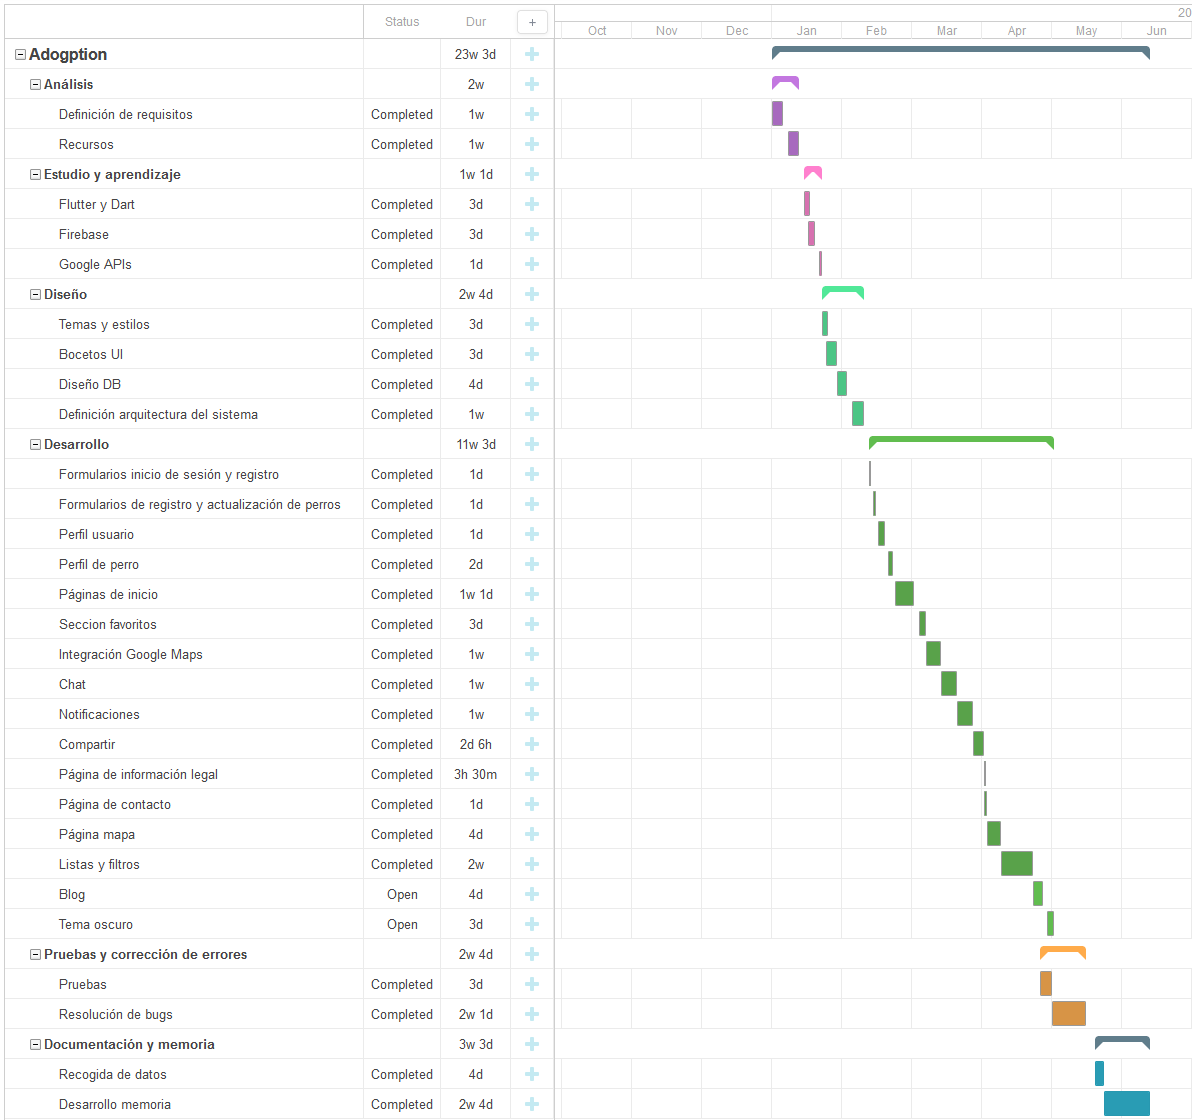
\includegraphics[width=15cm]{GanntSmall2.png}\par}
	\caption{Diagrama de Gannt}
\end{figure}


% Análisis
\newpage
\section{Análisis}

% Definición y Especificación de Requisitos
\subsection{Definición y especificación de Requisitos}

Para garantizar buenos resultados a la hora de desarrollar la aplicación, es esencial definir y comprender los requisitos que guiarán la creación y el diseño del sistema. Estos requisitos se dividen en dos categorías principales: requisitos funcionales y requisitos no funcionales.

En esta sección, se detallan tanto los requisitos funcionales como los no funcionales identificados para la aplicación en desarrollo. 

\subsubsection{Requisitos funcionales}

Los requisitos funcionales describen las acciones específicas que el sistema debe realizar, los servicios que debe proporcionar y cómo debe responder a diversas entradas. Estos requisitos se centran en el "qué" del sistema, delineando las funcionalidades clave que los usuarios esperan encontrar en la aplicación.

% RF1
\begin{table}[H]
\captionsetup{justification=raggedright,singlelinecheck=false}
\caption{\textbf{RF1:} Registro de usuarios y protectoras.}
\label{tab:RF1}
	\begin{tabular}{|m{5cm}|m{10cm}|}
	\hline
	\textbf{Explicación} & Proporcionar formularios de registro para usuarios y protectoras. \\ 
	\hline
	\textbf{Datos de Entrada} & Datos ingresados por el usuario en el formulario de registro. Incluyendo datos de contacto, correo electrónico y dirección \\ 
	\hline
	\textbf{Datos de Salida} & Datos del usuario almacenados en la base de datos. \\ 
	\hline
\end{tabular}
\end{table}

% RF2
\begin{table}[H]
\captionsetup{justification=raggedright,singlelinecheck=false}
\caption{\textbf{RF2:} Registro de caninos.}
\label{tab:RF2}
	\begin{tabular}{|m{5cm}|m{10cm}|}
	\hline
	\textbf{Explicación} & Ofrecer un formulario de registro para añadir perros con características específicas. \\ 
	\hline
	\textbf{Datos de Entrada} & Datos ingresados por la protectora, tales como raza, peso, edad, color y descripción. \\ 
	\hline
	\textbf{Datos de Salida} & Datos del perro almacenados en la base de datos, junto al id de su protectora. \\ 
	\hline
\end{tabular}
\end{table}

% RF3
\begin{table}[H]
\captionsetup{justification=raggedright,singlelinecheck=false}
\caption{\textbf{RF3:} Mostrar listas de usuarios.}
\label{tab:RF23}
	\begin{tabular}{|m{5cm}|m{10cm}|}
	\hline
	\textbf{Explicación} & Mostrar diferentes listas de usuarios en la aplicación, con filtros predeterminados. \\ 
	\hline
	\textbf{Datos de Entrada} & Ninguno. \\ 
	\hline
	\textbf{Datos de Salida} & Listas de usuarios de la aplicación que cumplen con los filtros.  \\ 
	\hline
\end{tabular}
\end{table}

% RF4
\begin{table}[H]
\captionsetup{justification=raggedright,singlelinecheck=false}
\caption{\textbf{RF4:} Mostrar listas de perros.}
\label{tab:RF4}
	\begin{tabular}{|m{5cm}|m{10cm}|}
	\hline
	\textbf{Explicación} & Mostrar diferentes listas de perros en la aplicación, con filtros predeterminados \\ 
	\hline
	\textbf{Datos de Entrada} & Ninguno. \\ 
	\hline
	\textbf{Datos de Salida} & Listas de perros de la aplicación que cumplen con los filtros. \\ 
	\hline
\end{tabular}
\end{table}

% RF5
\begin{table}[H]
\captionsetup{justification=raggedright,singlelinecheck=false}
\caption{\textbf{RF5:} Capacidad de filtrado por propiedades en listas de perros.}
\label{tab:RF5}
	\begin{tabular}{|m{5cm}|m{10cm}|}
	\hline
	\textbf{Explicación} & Proporcionar diferentes filtros para las listas de perros, que corresponden con las diferentes propiedades que puede tener un perro en la aplicación. \\ 
	\hline
	\textbf{Datos de Entrada} & Valores de los filtros proporcionados por el usuario. \\ 
	\hline
	\textbf{Datos de Salida} & Lista de perros de la aplicación que cumplen con los filtros. \\ 
	\hline
\end{tabular}
\end{table}

% RF6
\begin{table}[H]
\captionsetup{justification=raggedright,singlelinecheck=false}
\caption{\textbf{RF6:} Capacidad de filtrado por búsqueda en listas de perros.}
\label{tab:RF6}
	\begin{tabular}{|m{5cm}|m{10cm}|}
	\hline
	\textbf{Explicación} & Filtrar resultados de listas según el texto ingresado en una barra de búsqueda, la búsqueda se realiza en diferentes campos de los perros. \\ 
	\hline
	\textbf{Datos de Entrada} & Texto de búsqueda ingresado por el usuario. \\ 
	\hline
	\textbf{Datos de Salida} &  Lista de perros de la aplicación que cumplen con el criterio de búsqueda en alguno de los campos. \\ 
	\hline
\end{tabular}
\end{table}

% RF7
\begin{table}[H]
\captionsetup{justification=raggedright,singlelinecheck=false}
\caption{\textbf{RF7:} Capacidad de filtrado por búsqueda en listas de usuarios..}
\label{tab:RF7}
	\begin{tabular}{|m{5cm}|m{10cm}|}
\hline
	\textbf{Explicación} & Filtrar resultados de listas según el texto ingresado en una barra de búsqueda, la búsqueda se realiza en diferentes campos de los usuarios. \\ 
	\hline
	\textbf{Datos de Entrada} & Texto de búsqueda ingresado por el usuario. \\ 
	\hline
	\textbf{Datos de Salida} &  Lista de usuarios de la aplicación que cumplen con el criterio de búsqueda en alguno de los campos. \\ 
	\hline
\end{tabular}
\end{table}

% RF8
\begin{table}[H]
\captionsetup{justification=raggedright,singlelinecheck=false}
\caption{\textbf{RF8:}  Proporcionar botón de mapa de resultados en listas de usuarios.}
\label{tab:RF8}
	\begin{tabular}{|m{5cm}|m{10cm}|}
	\hline
	\textbf{Explicación} & Botón en listas de usuarios que redirige a una página con mapa con todos los resultados con ubicación. \\ 
	\hline
	\textbf{Datos de Entrada} & Ninguno \\ 
	\hline
	\textbf{Datos de Salida} & Botón con capacidad de redirección a la página del mapa. \\ 
	\hline
\end{tabular}
\end{table}

% RF9
\begin{table}[H]
\captionsetup{justification=raggedright,singlelinecheck=false}
\caption{\textbf{RF9:} Proporcionar botón de favoritos en perfiles de perros.}
\label{tab:RF9}
	\begin{tabular}{|m{5cm}|m{10cm}|}
	\hline
	\textbf{Explicación} & Permitir a un usuario o protectora marcar como favorito a un perro. \\ 
	\hline
	\textbf{Datos de Entrada} & Click del usuario sobre el botón. \\ 
	\hline
	\textbf{Datos de Salida} & Datos del perro con la actualización de ids de usuarios que lo han marcado/desmarcado como favorito.\\ 
	\hline
\end{tabular}
\end{table}

% RF10
\begin{table}[H]
\captionsetup{justification=raggedright,singlelinecheck=false}
\caption{\textbf{RF10:} Mostrar sección de perros favoritos. }
\label{tab:RF10}
	\begin{tabular}{|m{5cm}|m{10cm}|}
	\hline
	\textbf{Explicación} & Muestra una sección de perros marcados como favoritos en ese momento por el usuario en su página de inicio. \\ 
	\hline
	\textbf{Datos de Entrada} & Ninguno. \\ 
	\hline
	\textbf{Datos de Salida} & Lista horizontal de perros favoritos en la parte inferiro de la página de inicio de los usuarios. \\ 
	\hline
\end{tabular}
\end{table}

% RF11
\begin{table}[H]
\captionsetup{justification=raggedright,singlelinecheck=false}
\caption{\textbf{RF11:} Mostrar adopciones recientes.}
\label{tab:RF11}
	\begin{tabular}{|m{5cm}|m{10cm}|}
	\hline
	\textbf{Explicación} & Muestra un swiper con imágenes de perros marcados como adoptados recientemente. \\ 
	\hline
	\textbf{Datos de Entrada} & Ninguno. \\ 
	\hline
	\textbf{Datos de Salida} & Swiper con imágenes y nombres de perros adoptados en la aplicación. \\ 
	\hline
\end{tabular}
\end{table}

% RF12
\begin{table}[H]
\captionsetup{justification=raggedright,singlelinecheck=false}
\caption{\textbf{RF12:} Proporcionar botón de cerrar sesión.}
\label{tab:RF12}
	\begin{tabular}{|m{5cm}|m{10cm}|}
	\hline
	\textbf{Explicación} & Mostrar botón de cerrar sesión en el menú de acciones en la app bar de la aplicación. \\ 
	\hline
	\textbf{Datos de Entrada} & Ninguno. \\ 
	\hline
	\textbf{Datos de Salida} & Mostrar página de inicio de sesión, después de haber eliminado todos los datos relacionados con el usuario iniciado. \\ 
	\hline
\end{tabular}
\end{table}

% RF13
\begin{table}[H]
\captionsetup{justification=raggedright,singlelinecheck=false}
\caption{\textbf{RF13:} Proporcionar botón de contacto.}
\label{tab:RF13}
	\begin{tabular}{|m{5cm}|m{10cm}|}
	\hline
	\textbf{Explicación} & Mostrar botón de contacto en el menú de acciones en la app bar de la aplicación. \\ 
	\hline
	\textbf{Datos de Entrada} & Ninguno. \\ 
	\hline
	\textbf{Datos de Salida} & Mostrar página de contacto. \\ 
	\hline
\end{tabular}
\end{table}

% RF14
\begin{table}[H]
\captionsetup{justification=raggedright,singlelinecheck=false}
\caption{\textbf{RF14:} Botón de menu lateral en la app bar.}
\label{tab:RF14}
	\begin{tabular}{|m{5cm}|m{10cm}|}
	\hline
	\textbf{Explicación} & Mostrar botón que abre menú lateral. \\ 
	\hline
	\textbf{Datos de Entrada} & Ninguno. \\ 
	\hline
	\textbf{Datos de Salida} & Menu lateral con las páginas disponibles para ese usuario. \\ 
	\hline
\end{tabular}
\end{table}

% RF15
\begin{table}[H]
\captionsetup{justification=raggedright,singlelinecheck=false}
\caption{\textbf{RF15:} Mostrar datos personales en el menú lateral.}
\label{tab:RF15}
	\begin{tabular}{|m{5cm}|m{10cm}|}
	\hline
	\textbf{Explicación} & Muestra los datos del usuario iniciado en el menú lateral. \\ 
	\hline
	\textbf{Datos de Entrada} & Ninguno. \\ 
	\hline
	\textbf{Datos de Salida} & Datos del usuario almacenados en la base de datos. \\ 
	\hline
\end{tabular}
\end{table}

% RF16
\begin{table}[H]
\captionsetup{justification=raggedright,singlelinecheck=false}
\caption{\textbf{RF16:} Botón de 'Inicio' en el menú lateral.}
\label{tab:RF16}
	\begin{tabular}{|m{5cm}|m{10cm}|}
	\hline
	\textbf{Explicación} & Proporcionar botón para redirigir al usuario a la página de inicio de la aplicación. \\ 
	\hline
	\textbf{Datos de Entrada} &  Ninguno. \\ 
	\hline
	\textbf{Datos de Salida} &  Página de inicio de la aplicación. \\ 
	\hline
\end{tabular}
\end{table}

% RF17
\begin{table}[H]
\captionsetup{justification=raggedright,singlelinecheck=false}
\caption{\textbf{RF17:} Botón de 'Perfil personal' en el menú lateral.}
\label{tab:RF17}
	\begin{tabular}{|m{5cm}|m{10cm}|}
	\hline
	\textbf{Explicación} & Proporcionar botón para redirigir al usuario a la página de inicio de la aplicación. \\ 
	\hline
	\textbf{Datos de Entrada} &  Ninguno. \\ 
	\hline
	\textbf{Datos de Salida} &  Página de perfil personal. \\ 
	\hline
	\hline
\end{tabular}
\end{table}

% RF18
\begin{table}[H]
\captionsetup{justification=raggedright,singlelinecheck=false}
\caption{\textbf{RF18:} Botón de 'Mensajes' en el menú lateral.}
\label{tab:RF18}
	\begin{tabular}{|m{5cm}|m{10cm}|}
	\hline
	\textbf{Explicación} & Proporcionar botón para redirigir al usuario a la página de chats de la aplicación. \\ 
	\hline
	\textbf{Datos de Entrada} &  Ninguno. \\ 
	\hline
	\textbf{Datos de Salida} &  Página de chats. \\ 
	\hline
\end{tabular}
\end{table}

% RF19
\begin{table}[H]
\captionsetup{justification=raggedright,singlelinecheck=false}
\caption{\textbf{RF19:} Botón de 'Protectoras' en el menú lateral.}
\label{tab:RF19}
	\begin{tabular}{|m{5cm}|m{10cm}|}
	\hline
	\textbf{Explicación} & Proporcionar botón para redirigir al usuario a la lista de protectoras de la aplicación. \\ 
	\hline
	\textbf{Datos de Entrada} &  Ninguno. \\ 
	\hline
	\textbf{Datos de Salida} &  Lista de protectoras ya verificadas en la aplicación. \\ 
	\hline
\end{tabular}
\end{table}

% RF20
\begin{table}[H]
\captionsetup{justification=raggedright,singlelinecheck=false}
\caption{\textbf{RF20:} Botón de 'Mis perros' en el menú lateral.}
\label{tab:RF20}
	\begin{tabular}{|m{5cm}|m{10cm}|}
	\hline
	\textbf{Explicación} & Proporcionar botón para redirigir al usuario a la lista de sus perros de la aplicación \\ 
	\hline
	\textbf{Datos de Entrada} &  Ninguno. \\ 
	\hline
	\textbf{Datos de Salida} &  Lista de perros que ha dado de alta el usuario en la aplicación. \\ 
	\hline
\end{tabular}
\end{table}

% RF21
\begin{table}[H]
\captionsetup{justification=raggedright,singlelinecheck=false}
\caption{\textbf{RF21:} Botón de 'Usuarios' en el menú lateral.}
\label{tab:RF21}
	\begin{tabular}{|m{5cm}|m{10cm}|}
	\hline
	\textbf{Explicación} & Proporcionar botón para redirigir al usuario a la lista de usuarios de la aplicación. \\ 
	\hline
	\textbf{Datos de Entrada} &  Ninguno. \\ 
	\hline
	\textbf{Datos de Salida} &  Lista de usuarios que no son protectoras en la aplicación. \\ 
	\hline
\end{tabular}
\end{table}

% RF22
\begin{table}[H]
\captionsetup{justification=raggedright,singlelinecheck=false}
\caption{\textbf{RF22:} Botón de 'Información legal' en el menú lateral.}
\label{tab:RF22}
	\begin{tabular}{|m{5cm}|m{10cm}|}
	\hline
	\textbf{Explicación} & Proporcionar botón para redirigir al usuario a la página de información legal de la aplicación. \\ 
	\hline
	\textbf{Datos de Entrada} &  Ninguno. \\ 
	\hline
	\textbf{Datos de Salida} &  Página de información legal de la aplicación. \\ 
	\hline
\end{tabular}
\end{table}

% RF23
\begin{table}[H]
\captionsetup{justification=raggedright,singlelinecheck=false}
\caption{\textbf{RF23:} Edición de datos personales y de contacto.}
\label{tab:RF23}
	\begin{tabular}{|m{5cm}|m{10cm}|}
	\hline
	\textbf{Explicación} & Proporcionar formularios de edición para los datos del usuario. \\ 
	\hline
	\textbf{Datos de Entrada} & Datos ingresados por el usuario en el formulario. Puede haber datos sin actualizar. \\ 
	\hline
	\textbf{Datos de Salida} &  Datos del usuario actualizados en la base de datos. \\ 
	\hline
\end{tabular}
\end{table}

% RF24
\begin{table}[H]
\captionsetup{justification=raggedright,singlelinecheck=false}
\caption{\textbf{RF24:} Edición de datos de perros.}
\label{tab:RF24}
	\begin{tabular}{|m{5cm}|m{10cm}|}
	\hline
	\textbf{Explicación} & Propocionar formularios de edición para los datos de los caninos. \\ 
	\hline
	\textbf{Datos de Entrada} &  Datos ingresados por el usuario en el formulario. Puede haber datos sin actualizar.  \\ 
	\hline
	\textbf{Datos de Salida} &   Datos del canino actualizados en la base de datos. \\ 
	\hline
\end{tabular}
\end{table}

% RF25
\begin{table}[H]
\captionsetup{justification=raggedright,singlelinecheck=false}
\caption{\textbf{RF25:} Recuperación de contraseña.}
\label{tab:RF25}
	\begin{tabular}{|m{5cm}|m{10cm}|}
	\hline
	\textbf{Explicación} & Proporcionar formularios de recuperación de contraseña para los usuarios y protectoras. \\ 
	\hline
	\textbf{Datos de Entrada} & Correo electrónico ingresado por el usuario. \\ 
	\hline
	\textbf{Datos de Salida} & Correo electrónico con las instrucciones de recuperación de contraseña. \\ 
	\hline
\end{tabular}
\end{table}

% RF26
\begin{table}[H]
\captionsetup{justification=raggedright,singlelinecheck=false}
\caption{\textbf{RF26:} Mostrar página de perfil de usuario/protectora.}
\label{tab:RF26}
	\begin{tabular}{|m{5cm}|m{10cm}|}
	\hline
	\textbf{Explicación} & Proporcionar una interfaz que condense toda la información de un usuario en una sola página. \\ 
	\hline
	\textbf{Datos de Entrada} & Ninguno. \\ 
	\hline
	\textbf{Datos de Salida} & Datos del usuario correspondinte, incluyendo foto de perfil, correo y los perros (si los tiene). Además incluirá el botón de contacto para abir chat. \\ 
	\hline
\end{tabular}
\end{table}

% RF27
\begin{table}[H]
\captionsetup{justification=raggedright,singlelinecheck=false}
\caption{\textbf{RF27:} Mostrar página de perfil de canino.}
\label{tab:RF27}
	\begin{tabular}{|m{5cm}|m{10cm}|}
	\hline
	\textbf{Explicación} & Proporcionar una interfaz que condense toda la información relacionada con un perro en una sola página. \\ 
	\hline
	\textbf{Datos de Entrada} & Ninguno. \\ 
	\hline
	\textbf{Datos de Salida} & Datos del perro correspondiente, incluyendo foto de perfil, características del canino (edad, raza, peso, descripción...). Además de un mapa indicando su ubicación, el bóton de favoritos y de compartir. También incluye el botón de abrir chat. Contendrá los botones de edición si el perro es del usuario que visita el perfil. \\ 
	\hline
\end{tabular}
\end{table}

% RF28
\begin{table}[H]
\captionsetup{justification=raggedright,singlelinecheck=false}
\caption{\textbf{RF28:} Compartir perros a través de enlace.}
\label{tab:RF28}
	\begin{tabular}{|m{5cm}|m{10cm}|}
	\hline
	\textbf{Explicación} & Proporcionar un botón que genere un enlace para redirigir a un usuario al perfil de ese perro en concreto. \\ 
	\hline
	\textbf{Datos de Entrada} & Ninguno. \\ 
	\hline
	\textbf{Datos de Salida} & Url a la aplicación con los parámetros correspondientes para redirigir al perfil de perro. \\ 
	\hline
\end{tabular}
\end{table}

% RF29
\begin{table}[H]
\captionsetup{justification=raggedright,singlelinecheck=false}
\caption{\textbf{RF29:} Página del mapa.}
\label{tab:RF29}
	\begin{tabular}{|m{5cm}|m{10cm}|}
	\hline
	\textbf{Explicación} & Proporcionar una interfaz que contenga un mapa con diferentes marcadores para cada una de las protectoras y un listado de las mismas debajo del mapa. \\ 
	\hline
	\textbf{Datos de Entrada} & Ninguno. \\ 
	\hline
	\textbf{Datos de Salida} & Mapa con marcadores y listado de protectoras, con elementos que pueden mover la cámara a los diferentes marcadores del mapa. \\ 
	\hline
\end{tabular}
\end{table}


% RF30
\begin{table}[H]
\captionsetup{justification=raggedright,singlelinecheck=false}
\caption{\textbf{RF30:} Página de chats.}
\label{tab:RF30}
	\begin{tabular}{|m{5cm}|m{10cm}|}
	\hline
	\textbf{Explicación} & Proporcionar una interfaz que contenga un listado de chats abiertos dentro de la aplicación. \\ 
	\hline
	\textbf{Datos de Entrada} & Ninguno. \\ 
	\hline
	\textbf{Datos de Salida} & Listado de chats disponibles en la aplicación, incluyen una preview del último mensaje y datos del usuario correspondiente. \\ 
	\hline
\end{tabular}
\end{table}


% RF31
\begin{table}[H]
\captionsetup{justification=raggedright,singlelinecheck=false}
\caption{\textbf{RF31:} Enviar mensajes al chat.}
\label{tab:RF31}
	\begin{tabular}{|m{5cm}|m{10cm}|}
	\hline
	\textbf{Explicación} & Permitir mandar mensajes a otro usuario dentro de la aplicación. \\ 
	\hline
	\textbf{Datos de Entrada} & Texto ingresado por el usuario. \\ 
	\hline
	\textbf{Datos de Salida} & Mensaje guardado en la base de datos Se ctualizar la tabla de chats de la base de datos con el último mensaje enviado y generar el id del chat si es el primer mensaje. Notificación al usuario receptor. \\ 
	\hline
\end{tabular}
\end{table}


% RF32
\begin{table}[H]
\captionsetup{justification=raggedright,singlelinecheck=false}
\caption{\textbf{RF32:} Enviar imágenes al chat.}
\label{tab:RF32}
	\begin{tabular}{|m{5cm}|m{10cm}|}
\hline
	\textbf{Explicación} & Permitir mandar mensajes a otro usuario dentro de la aplicación. \\ 
	\hline
	\textbf{Datos de Entrada} & Imagen adjuntada por el usuario. \\ 
	\hline
	\textbf{Datos de Salida} & Imagen guardada además de su referencia en la tabla de mensaje. Se la tabla de chats de la base de datos con el último mensaje enviado y generar el id del chat si es el primer mensaje. Notificación al usuario receptor. \\ 
	\hline
\end{tabular}
\end{table}


% RF33
\begin{table}[H]
\captionsetup{justification=raggedright,singlelinecheck=false}
\caption{\textbf{RF33:} Abrir un chat nuevo.}
\label{tab:RF33}
	\begin{tabular}{|m{5cm}|m{10cm}|}
	\hline
	\textbf{Explicación} & Proporcionar un botón de contacto para abrir un chat con algún usuario dentro de la aplicación. \\ 
	\hline
	\textbf{Datos de Entrada} & Ninguno. \\ 
	\hline
	\textbf{Datos de Salida} & Interfaz del chat, con la cabecera que incluye los datos del usuario receptor. \\ 
	\hline
\end{tabular}
\end{table}

% RF34
\begin{table}[H]
\captionsetup{justification=raggedright,singlelinecheck=false}
\caption{\textbf{RF34:} Borrar un chat.}
\label{tab:RF34}
	\begin{tabular}{|m{5cm}|m{10cm}|}
	\hline
	\textbf{Explicación} & Deslizar un chat para eliminarlo de la lista de chats disponibles \\ 
	\hline
	\textbf{Datos de Entrada} & Ninguno. \\ 
	\hline
	\textbf{Datos de Salida} & Lista actualizada sin el chat que se acaba de eliminar \\ 
	\hline
\end{tabular}
\end{table}

% RF35
\begin{table}[H]
\captionsetup{justification=raggedright,singlelinecheck=false}
\caption{\textbf{RF35:} Marcar/desmarcar perro como adoptado.}
\label{tab:RF35}
	\begin{tabular}{|m{5cm}|m{10cm}|}
	\hline
	\textbf{Explicación} & Proporcionar un botón dentro del perfil del perro que permite a una protectora marcar/desmarcar a un perro de la aplicación como adoptado. \\ 
	\hline
	\textbf{Datos de Entrada} & Estado nuevo según si se quiere marcar o desmarcar. \\ 
	\hline
	\textbf{Datos de Salida} & Perfil del canino actualizado y una etiqueta que indica si está adoptado. \\ 
	\hline
\end{tabular}
\end{table}


% RF36
\begin{table}[H]
\captionsetup{justification=raggedright,singlelinecheck=false}
\caption{\textbf{RF36:} Página de contacto.}
\label{tab:RF36}
	\begin{tabular}{|m{5cm}|m{10cm}|}
	\hline
	\textbf{Explicación} & Proporcionar una interfaz que rehúna datos de contacto de administradores. \\ 
	\hline
	\textbf{Datos de Entrada} & Ninguno. \\ 
	\hline
	\textbf{Datos de Salida} & Interfaz que incluye correo electrónico y un botón de contacto para abrir un chat con un administrador. \\ 
	\hline
\end{tabular}
\end{table}

% RF37
\begin{table}[H]
\captionsetup{justification=raggedright,singlelinecheck=false}
\caption{\textbf{RF37:} Página de información legal.}
\label{tab:RF37}
	\begin{tabular}{|m{5cm}|m{10cm}|}
	\hline
	\textbf{Explicación} & Proporcionar una interfaz que rehúna toda la información legal y advertencias. \\ 
	\hline
	\textbf{Datos de Entrada} & Ninguno. \\ 
	\hline
	\textbf{Datos de Salida} & Interfaz que incluye toda la información legal de la aplicación. \\ 
	\hline
\end{tabular}
\end{table}

% RF38
\begin{table}[H]
\captionsetup{justification=raggedright,singlelinecheck=false}
\caption{\textbf{RF38:} Proporcionar página de inició según rol.}
\label{tab:RF38}
	\begin{tabular}{|m{5cm}|m{10cm}|}
	\hline
	\textbf{Explicación} & Proporcionar una interfaz única según el rol después de iniciar sesión. \\ 
	\hline
	\textbf{Datos de Entrada} & Correo electrónico y contraseña para iniciar sesión. \\ 
	\hline
	\textbf{Datos de Salida} & Página de inicio que varía según el rol. \\ 
	\hline
\end{tabular}
\end{table}

% RF39
\begin{table}[H]
\captionsetup{justification=raggedright,singlelinecheck=false}
\caption{\textbf{RF39:} Página de administrador.}
\label{tab:RF39}
	\begin{tabular}{|m{5cm}|m{10cm}|}
	\hline
	\textbf{Explicación} & Proporcionar una página para los administradores. \\ 
	\hline
	\textbf{Datos de Entrada} & Correo electrónico y contraseña de administrador para iniciar sesión. \\ 
	\hline
	\textbf{Datos de Salida} & Interfaz para los administradores, que incluye listas con diferentes filtros de usuarios y caninos para manejar usuarios y caninos. \\ 
	\hline
\end{tabular}
\end{table}

% RF40
\begin{table}[H]
\captionsetup{justification=raggedright,singlelinecheck=false}
\caption{\textbf{RF40:} Búsqueda de direcciones.}
\label{tab:RF40}
	\begin{tabular}{|m{5cm}|m{10cm}|}
	\hline
	\textbf{Explicación} & Proporcionar una barra de búsqueda de direcciones para facilitar la introducción de datos. \\ 
	\hline
	\textbf{Datos de Entrada} & Una cadena de caracteres que puede contener el nombre de la calle, la ciudad, el código postal... \\ 
	\hline
	\textbf{Datos de Salida} & Un listado de direcciones que coinciden con la búsqueda, al seleccionar una, se autocompletan los datos del formulario. \\ 
	\hline
\end{tabular}
\end{table}


\subsubsection{Requisitos no funcionales}

Los requisitos no funcionales son los encargados de ofrecer al usuario una experiencia robusta y óptima a lo largo de la aplicación. Para el desarrollo de la aplicación se han tenido en cuenta los siguientes puntos:

\begin{itemize}
	\item \textbf{Rendimiento:} La aplicación debe ser capaz de responder rápidamente a las interacciones de los usuarios y ejecutar las operaciones en un breve período de tiempo. Aquí se listan las propuestas a tener en cuenta a la hora de desarrollar.
		\begin{itemize}
			\item Se propone una deadline de 3 segundos como tiempo óptimo para cargar una página completa.
			\item El tiempo de respuesta del servidor se espera que sea menor de 2 segundos.
			\item Se espera que la aplicación sea capaz de manejar múltiples peticiones sin que se produzca una degradación perceptible del rendimiento. Se propone como deadline 10000 de solicitudes.
			\item Se espera que la base de datos realice consultas simples y complejas en menos de un segundo.
			\item Se propone que en el caso de búsquedas y filtrados el tiempo de procesamiento puede ser mayor de 3 segundos, pero menor de 6.
			\item La aplicación denbe poder manejar alrededor de 10000 usuarios de forma concurrente sin sufrir degradación de rendimiento.
		\end{itemize}
	\item \textbf{Escalabilidad:} Es necesario que a la hora de implementar código, se mantenga un código en el que sea sencillo añadir o quitar funcionalidades sin comprometer el comportamiento de la aplicación.
		\begin{itemize}
			\item Los componentes de la aplicación deben estar claramente definidos y documentados.
			\item Un componente base debe recoger todas las propiedades comunes que pueden tener ese tipo de componentes. Por ejemplo, un componente base para los botones, deberá recoger el tamaño de la fuente, la forma del botón, colores etc.
			\item Las funcionalidades desarrolladas deben ser fácilmente deprecadas si es necesario, es decir, no deben depender unas de otras si no es estrictamente necesario.
			\item Los nuevos componentes que se desarrollen no deben afectar el funcionamiento de la aplicación.
			\item Se espera que si fuera necesario actualizar algún componente en la UI, actualizando el componente base se actualicen todos los componentes de ese tipo.
		\end{itemize}
	\item \textbf{Usabilidad:} Para esta aplicación, como tiene un rango de usuarios muy amplio, se espera que un usuario poco experimentado sea capaz de usar la aplicación de form sencilla. La aplicación debe proporcionar una interfaz intuitiva y atractiva. 
		\begin{itemize}
			\item La interfaz debe ser limpia y organizada.
			\item Los colores de la aplicación deben ser coherentes.
			\item La navegación de la aplicación debe cumplir la norma de los tres clicks, "\textit{cualquier persona que visite nuestro sitio debería alcanzar la información más crítica como máximo en tres clics}".
			\item La aplicación deberá ser lo suficientemente intuitiva o proporcionar guía de uso si es necesario.
			\item Se espera que la aplicación sea testeada por usuarios reales antes del primer despliegue para posibles correciones.
		\end{itemize}
	\item \textbf{Confiabilidad:} Para la aplicación, se espera que haya un correcto manejo de errores.
		\begin{itemize}
			\item Se espera que un usuario sea informado con un mensaje adecuado si ocurre un error crítico.
			\item Durante el desarrollo es necesario testear para poder añadir mecanismos que minimicen los errores conocidos en la aplicación.
			\item Las copias de seguridad son indispensables para garantizar que no se pierden los datos ante un error crítico.
			\item Se propone añadir mecanismos de manejo de errores en todas las operaciones críticas (lectura y escritura)  para evitar errores críticos.
		\end{itemize}
	\item \textbf{Seguridad:} Para garantizar este requisito, la aplicación debe proteger los datos de los usuarios y prevenir accesos no autorizados. También, en este caso en concreto, es necesario garantizar en medida de los posible, que toda la información que se dé de alta, sea real y fehaciente.
		\begin{itemize}
			\item Las contraseñas o datos sensibles no pueden estar expuestos, se deben almacenar con cifrados.
			\item La aplicación no va a permitir el acceso a usuarios que no tengan una cuenta.
			\item La aplicación no va a permitir dar de alta a perros a las protectoras que no estén verificadas por administradores, para evitar casos fraudulentos.
			\item Un administrador tiene acceso a diferentes listas en las que puede verificar información y tiene la libertad de eliminar lo que crea correspondiente.
			\item Debe prevenirse con mecanismos para ataques comunes como pueden ser las inyecciones SQL, CSS, Y CSRF. 
		\end{itemize}
	\item \textbf{Documentación:} A lo largo de todas las etapas, se almacenará toda la información relevante, ya sea en el código, en documentos aparte o en la propia memoria.
\end{itemize}

% Recursos
\subsection{Recursos}
Posterior a definir todos los requisitos de la aplicación, se pude concretar que va a ser necesario utilizar durante el desarrollo del proyecto, tanto mano de obra, como hardware y software.

\subsubsection{Recursos humanos}

En este proyecto, solo va a intervenir una persona, la autora de la memoria. Se trata de una Ingeniera de Software (semi-senior). Es encargada de cumplimentar todos los puntos del desarrollo. El horario laboral sería de Lunes a Viernes de media jornada.


\subsubsection{Hardware}

Para este proyecto el hardware es un ordenador de sobremesa personal

\begin{itemize}
	\item Ordenador de sobremesa, para el desarrollo y las pruebas, con los siguientes componentes:
		\begin{itemize}
			\item \textbf{Procesador:} AMD Ryzen 7 3700X 8-Core Processor - 3.60 GHz
			\item \textbf{Memoria RAM:} DDR4 3000 2x16GB
			\item \textbf{Tarjeta gráfica:} NVIDIA GeForce GTX 1660 SUPER
			\item \textbf{Placa base:} ASUS TUF GAMING B550-PLUS WIFI II
			\item \textbf{Disipador:} Noctua NH-D15
		\end{itemize}
	\item Tablet android Hi9plus, para realizar pruebas en un dispositivo android físico.
\end{itemize}

\subsubsection{Software}

El sistema operativo utilizado es el que estaba instalado previamente en el ordenador personal.

Para escoger el framework que se va a utilizar en el proyecto partimos de la base de que vamos a realizar una aplicación android. Existen diferentes frameworks como \textit{React Native}, \textit{Flutter}, \textit{Kotlin Multiplatform} etc. que ofrecen integración con android para facilitar el desarrollo. En este proyecto, se ha optado por desarrollar con Flutter, debido a que se ha trabajado previamente con él. Este framework, además, permite realizar un desarrollo multiplataforma y ofrece un alto rendimiento. 

El lenguaje utilizado es \textit{Dart}, este lenguaje es muy similar a Java, se trata de un lenguaje orientado a objetos y se utiliza prinicpalmente para el desarrollo de aplicaciones del lado del cliente. Es un lenguaje bastante popularizado, uno de los motivos de optar por este lenguaje, es el manenimiento que recibe a día de hoy y por la simple que resulta para programar. Para añadir funcionalidades extra, se han escogido varias bibiliotecas que ofrecen algunos microservicios o widgets.

Por último, para manejar la base de datos, entre otros, se ha optado por usar \textit{Firebase}. Se trata de una plataforma de desarrollo de aplicaciones web muy popularizada, también desarrollada por Google. Ofrece diferentes servicios para la autenticación, el hosting de la aplicación y bases de datos en tiempo real, eso lo convertia en el candidato adecuado para manejar el chat, la funcionalidad de compartir entre otras cosas que nuestra aplicación requiere.

\begin{itemize}
	\item \textbf{Sistema Operativo:} Windows 11 x64
	\item \textbf{IDE:} Android Studio Hedgehog | 2023.1.1 Patch 2
	\item \textbf{Framework:} Flutter 3.19.0 -  \href{https://flutter.dev/6}{Flutter DEV}
	\item \textbf{Lenguaje:} Dart 3.3.0 - \href{https://dart.dev/}{Dart DEV}
	\item \textbf{Paquetes:}
		\begin{itemize}
		  \item \texttt{cupertino\_icons: \^{}1.0.2}
		  \item \texttt{firebase\_core: \^{}2.24.2}
		  \item \texttt{firebase\_database: \^{}10.3.8}
		  \item \texttt{firebase\_storage:}
		  \item \texttt{cloud\_firestore: \^{}4.13.6}
		  \item \texttt{firebase\_auth: \^{}4.15.3}
		  \item \texttt{responsive\_sizer: \^{}3.3.0+1}
		  \item \texttt{flutter\_login: \^{}5.0.0}
		  \item \texttt{google\_fonts: \^{}4.0.4}
		  \item \texttt{resize: \^{}1.0.0}
		  \item \texttt{awesome\_notifications: \^{}0.9.2}
		  \item \texttt{csc\_picker: \^{}0.2.7}
		  \item \texttt{map\_address\_picker: \^{}0.3.5}
		  \item \texttt{geocoding: \^{}3.0.0}
		  \item \texttt{search\_map\_location: 0.0.6}
		  \item \texttt{image\_picker: \^{}1.0.7}
		  \item \texttt{image\_cropper: \^{}4.0.1}
		  \item \texttt{path\_provider: \^{}2.1.2}
		  \item \texttt{flutter\_image\_compress: \^{}2.1.0}
		  \item \texttt{address\_form: \^{}0.0.2}
		  \item \texttt{address: \^{}0.1.0+2}
		  \item \texttt{google\_maps\_webservice: \^{}0.0.20-nullsafety.5}
		  \item \texttt{meta\_validator: \^{}0.0.2}
		  \item \texttt{geolocator: \^{}9.0.2}
		  \item \texttt{dropdown\_search: \^{}5.0.6}
		  \item \texttt{card\_swiper: \^{}3.0.1}
		  \item \texttt{filter\_list: \^{}1.0.2}
		  \item \texttt{flutter\_filter\_dialog: \^{}1.2.0}
		  \item \texttt{choice: \^{}2.3.2}
		  \item \texttt{animate\_gradient: \^{}0.0.2+1}
		  \item \texttt{firebase\_messaging: \^{}14.9.1}
		  \item \texttt{flutter\_chat\_bubble: \^{}2.0.2}
		  \item \texttt{chat\_bubbles: \^{}1.6.0}
		  \item \texttt{share\_plus: \^{}9.0.0}
		  \item \texttt{app\_links: \^{}6.0.1}
		  \item \texttt{url\_launcher: \^{}6.2.6}
		  \item \texttt{firebase\_dynamic\_links: \^{}5.5.4}
		  \item \texttt{go\_router: \^{}14.0.2}
		  \item \texttt{get: \^{}4.6.6}
		  \item \texttt{linkwell: \^{}2.0.6}
		  \item \texttt{toastification: \^{}1.0.0}
		\end{itemize}
	\item \textbf{Base de datos:} Firebase database - \href{https://console.firebase.google.com}{Firebase console}
\end{itemize}


\subsection{Costes}

Con la lista de recursos necesarios, ya se puede hacer un presupuesto de la aplicación adecuado según los diferentes apartados.

\subsubsection{Recursos humanos}

Para calcular el coste relacionado con el personal, se toma como referencia el sueldo medio de la persona involcurada en su trabajo actual, teniendo en cuenta que cobra entre los \textit{38.000€ } - \textit{43.000€ } anuales.

Tomando como media los \textit{40.000€ } anuales, al mes corresponden unos \textit{3.330€}. Como la duración del proyecto es de 5 meses y medio, el coste total en salarios para la empleada sería de \textit{18.315€}.

\subsubsection{Hardware}

Debido a que el equipo utilizado no es nuevo, consideraremos los gastos de estos teniendo en cuenta que un equipo informático se puede amortizar hasta 8 años. El precio aproximado del orenador es de unos \textit{1000€}.
Un año tiene 12 meses, así que tenemos 96 meses en total de amortización, lo que resulta a unos \textit{11€} al mes. Como la duración del proyecto es de 5 meses y medio, el coste del ordenador sería de \textit{60,50€}.

El precio de la tablet es de unos \textit{100€} así que con los mismos cálculos, el gasto de la tablet es de \textit{5,72€} en total.

\subsubsection{Software}

Para el alcance de este proyecto y los número a los que se aspira, al menos durante la primera fase, hemos optado por utilizar las versiones gratuitas del software implicado, lo que resulta en un coste total de 0€ en software.
\begin{itemize}
	\item Firebase - Plan Spark - \href{https://firebase.google.com/pricing?hl=es-419}{Guía de planes}
	\item Google APIs - Ofrecen créditos gratuitos de hasta \textit{200€} para cubir los gastos que se generen por el uso de la API. - \href{https://mapsplatform.google.com/intl/es/pricing/}{Precios}
	\item IDE + Framework - Gratuitos
\end{itemize}


\subsubsection{Otros}

Debido a que el desarrollo del proyecto se realiza en la casa de la persona empleada, se añaden a los costes la electricidad usada. Usando como referencia el gasto mensual de electricidad, que ronda los \textit{30€}, calculamos que van dirigidos a esta parte unos \textit{165€} extra.

\begin{table}[H]
    \centering
    \begin{tabular}{ | m{5cm} | m{5cm} | }
	    \hline \textbf{Recurso} & \textbf{Coste (€)} \\ \hline
	    	Personal & 18.315 \\ \hline
	    	\multirow{2}{*}{Hardware} & Ordenador - 60,50 \\& Tablet - 5,72 \\ \hline
	    	Software & 0 \\ \hline
	    \textbf{Total} & \textbf{18.381,22€} \\ \hline
    \end{tabular}
    \caption{Costes del proyecto}
    \label{tab:costes}
\end{table}

% Diseño
\newpage
\section{Diseño}

En esta parte tenemos que definir toda la estructura de la aplicación, tanto como la interfaz de usuario, el backend y la base de datos.

\subsection{Diseño de base de datos}

Esta sección es primordial para generar unas bases sólidas para la aplicación. Debemos almacenar distintas entidades y propiedades, consideramos las siguientes entidades y sus correspondientes tablas.

\subsubsection{Direcciones}

Para las protectoras almacenamos la dirección en la que están ubicadas. Esta dirección es necesaria para mostrar al usuario el texto de donde está y también para ubicarla en los mapas que se proporcionan en la app. Por una parte almacenamos la dirección por partes, incluyendo la ciudad, la calle, el código postal etc. Por otra parte, cuando generemos una dirección, a su vez guardaremos las coordenadas. Esta decisión se toma para evitar hacer cálculos repetidos cada vez que tengamos que cargar un mapa con marcadores, ya que estos requieren de las coordenadas geográficas directamente. Cuando se actualice una dirección, se actualizaran sus coordenadas.

Para todas las direcciónes se genera una entrada en el que su ID corresponde con el del usuario al que pertenece.

% Addresses
\begin{table}[H]
\captionsetup{justification=raggedright,singlelinecheck=false}
\caption{\textbf{Tabla: addresses}}
\label{tab:Addresses}
	\begin{tabular}{|m{3cm}|m{2cm}|m{5cm}|m{3cm}|}
	\hline
	\textbf{Campo} & \textbf{Tipo} & \textbf{Dato} & \textbf{Obligatorio} \\ 
	\hline
	\textbf{city} & cadena & Ciudad de la dirección & Si \\ 
	\hline
	\textbf{country} & cadena & País de la dirección (España siempre) & Si\\ 
	\hline
	\textbf{province} &  cadena & Provincia de la dirección & Si \\ 
	\hline
	\textbf{street} &  cadena & Calle de la dirección & Si \\ 
	\hline
	\textbf{street\_number} &  cadena & Número de la calle & No\\ 
	\hline
	\textbf{zipcode} & cadena & Código postal & Si \\ 
	\hline
	\textbf{lat} & número & Latitud & Si \\ 
	\hline
	\textbf{lng} & número & Longitud & Si \\ 
	\hline
\end{tabular}
\end{table}

Aqui se muestra un ejemplo real de una dirección almacenada en la base de datos.

\begin{verbatim}
{
  "city": "Murcia",
  "country": "España",
  "lat": 37.9879153,
  "lng": -1.1315578,
  "province": "Murcia",
  "street": "Calle Maestro Alonso",
  "street_number": "4",
  "zipcode": "30005"
}
\end{verbatim}

\subsubsection{Chats}

Para generar la tabla de chats, se decidió almacenar los ids de los usuarios implicados, aparte de para quién esta disponible el chat en ese momento. Esto es debido al requisito definido previamente en el que se define la posibilidad de eliminar un chat. Al igual que en otras aplicaciones de mensajería, cuando se elimina un chat, el chat simplemente desaparece para el usuario que lo borra, así que podemos actualizar la propiedad de para quien está visible el chat en ese momento. Para esta primera iteración del proyecto, los mensajes no se borran, así que si por ejemplo una persona A, borra su chat con la persona B, si vuelve a abrir un chat con esa persona, los mensajes anteriores aparecerán, en la parte de implementación de la memoria indagaremos más en profundidad acerca del comportamiento definido. 

Almacenar aqui los IDs de los usuarios implicados, permite que si se proponen chats de grupo, sea más sencillo escalarlo, ya que en esta forma la base de datos ya lo está soportando. Lo mismo ocurre con la propiedad que hace referencia a que usuarios pueden ver el chat. 

Para todos los chats se genera un ID automático, al que se hace referencia desde la tabla de usuarios.

% Chats
\begin{table}[H]
\captionsetup{justification=raggedright,singlelinecheck=false}
\caption{\textbf{Tabla: chats}}
\label{tab:chats}
	\begin{tabular}{|m{3cm}|m{2cm}|m{5cm}|m{3cm}|}
	\hline
	\textbf{Campo} & \textbf{Tipo} & \textbf{Dato} & \textbf{Obligatorio} \\ 
	\hline
	\textbf{availableTo} & array & IDs de Usuarios que tienen el chat visible en su página & Si \\ 
	\hline
	\textbf{lastMessage} & cadena & ID del último mensaje mandado en el chat & Si\\ 
	\hline
	\textbf{users} &  array & IDs de Usuarios que intervienen en el chat & Si \\ 
	\hline
\end{tabular}
\end{table}

Aqui se muestra un ejemplo real de un chat almacenado en la base de datos. 

\begin{verbatim}
{
  "availableTo": [
    "kuaKjc6XoiVot1rMeGqBySA5pE13",
    "buO4Vkazs3O2oVKetugxrvTfRw12"
  ],
  "lastMessage": "BaKmuuo8debUTdSNsvw0",
  "users": [
    "kuaKjc6XoiVot1rMeGqBySA5pE13",
    "buO4Vkazs3O2oVKetugxrvTfRw12"
  ]
}
\end{verbatim}

\subsubsection{Perros}

Esta entidad es una de las más importantes de la aplicación, ya que es la que se principal afectada por la mayoría de funcionalidades que se proponen. Principalmente esta tabla contendrá todas las propiedades de los perros que se van a manejar dentro de la app, aunque hay algunas consideraciones importantes para algunas de ellas. 

Para el género se han propuesto dos valores fijos que luego se transformaran en la cadena correspondiente cuando se carguen en la UI. Los valores son \textbf{male} y \textbf{female}. Se propone esta solución para cuando se decida añadir traducciones en la aplicación y no trabajar con palabras en Español en la base de datos.

Para almacenar la edad, se ha optado por almacenarla junto a las unidades, ya que así se le da la posibilidad al usuario a especificar mejor la edad del perro (el caso de uso es muy concreto, pero añade valor). Los valores de las unidades serán fijos, pudiendo ser:
	\begin{itemize}
		\item \textbf{Meses}
		\item \textbf{Años}
	\end{itemize}

Lo mismo ocurre con el peso, se opta por almacenar el peso junto con las unidades para facilitar al usuario especificar el peso. A pesar de que se pueda especificar las unidades del peso, el peso en la base de datos siempre será tratado como KG, para facilitar el uso de los filtros, cuando se traiga a la UI, se actualizará al valor real que corresponda. Las unidades disponibles serán
	\begin{itemize}
		\item \textbf{Gramos}
		\item \textbf{KG}
	\end{itemize}

En una primera instancia se propuso almacenar los perros favoritos en la tabla de usuarios, pero tras hacer algunas pruebas se optó por este modelo finalmente. Almacenar los usuarios que han marcado al perro como favorito, facilita las actualizaciones en tiempo real de los resultados de perros.

Para todos los perros se genera un ID automático.

\begin{table}[H]
\captionsetup{justification=raggedright,singlelinecheck=false}
\caption{\textbf{Tabla: dogs}}
\label{tab:dogs}
	\begin{tabular}{|m{3cm}|m{2cm}|m{5cm}|m{3cm}|}
	\hline
	\textbf{Campo} & \textbf{Tipo} & \textbf{Dato} & \textbf{Obligatorio} \\ 
	\hline
	\textbf{adopted} & booleano & Indica si el perro ha sido adoptado. & Si \\ 
	\hline
	\textbf{age} & número & Edad & Si \\ 
	\hline
	\textbf{ageUds} & cadena & Unidades de la edad & Si \\ 
	\hline
	\textbf{breed} & cadena & Raza & Si \\ 
	\hline
	\textbf{castrated} & booleano & Indica si está castrado & Si \\ 
	\hline
	\textbf{color} & cadena & Color & Si \\ 
	\hline
	\textbf{created} & marca de tiempo & Fecha y hora de cuando se ha dado de alta & Si \\ 
	\hline
	\textbf{description} & cadena & Descripción & No \\ 
	\hline
	\textbf{favoriteBy} & array & IDs de usuarios que lo han marcado como favorito & No \\ 
	\hline
	\textbf{forAdoption} & booleano & Indica si está disponible para adopción & No \\ 
	\hline
	\textbf{forFoster} & booleano & Indica si está disponible para acogida & No \\ 
	\hline
	\textbf{gender} & cadena & Género & Si \\ 
	\hline
	\textbf{name} & cadena & Nombre & Si \\ 
	\hline
	\textbf{ownerId} & cadena & ID del propietario & Si \\ 
	\hline
	\textbf{profilePic} & cadena & URL de la imagen de perfil de la mascota & No \\ 
	\hline
	\textbf{weight} & número & Peso & Si \\ 
	\hline
	\textbf{weightUds} & cadena & Unidades de peso & Si \\ 
	\hline
\end{tabular}
\end{table}

Aquí se muestra un ejemplo real de un perro almacenado en la base de datos.

\begin{verbatim}
{
  "adopted": false,
  "age": 1,
  "ageUds": "Años",
  "breed": "Breed 2",
  "castrated": true,
  "color": "Color 1",
  "created": "23 de abril de 2024, 10:56:48 a.m. UTC+2",
  "description": "",
  "favoriteBy": [],
  "forAdoption": true,
  "forFoster": true,
  "gender": "female",
  "name": "Katrina",
  "ownerId": "S4wXwckahiSOLI0Q3exXDVRh2yl2",
  "profilePic": "",
  "weight": 1,
  "weightUds": "KG"
}
\end{verbatim}

\subsubsection{Mensajes}

Aparte de almacenar toda la información de los chats, hay que almacenar los mensajes involucrados en los chats. Se propone guardar el tipo de mensaje, habiendo en esta primera iteración solo dos tipos, que serían \textbf{default} e \textbf{image}. Esta distinción es necesaria para cuando se cargue la preview del mensaje en la UI. Aparte, si el mensaje que se envía es una imagen, se generara una entrada para esa imagen.

Para todos los mensajes se genera un ID automático que se puede referenciar desde la tabla de chats.

% Mensajes
\begin{table}[H]
\captionsetup{justification=raggedright,singlelinecheck=false}
\caption{\textbf{Tabla: messages}}
\label{tab:messages}
	\begin{tabular}{|m{3.2cm}|m{2cm}|m{5cm}|m{3cm}|}
	\hline
	\textbf{Campo} & \textbf{Tipo} & \textbf{Dato} & \textbf{Obligatorio} \\ 
	\hline
	\textbf{chatId} & cadena & ID del chat & Si \\ 
	\hline
	\textbf{from} & cadena & ID del emisor del mensaje & Si \\ 
	\hline
	\textbf{messageContent} & cadena & Contenido del mensaje & Si \\ 
	\hline
	\textbf{read} & booleano & Indica si el recpetor a leído el mensaje & Si \\ 
	\hline
	\textbf{sent} & marca de tiempo & Fecha y hora en la que se mandó el mensaje & Si \\ 
	\hline
	\textbf{to} & cadena & ID del receptor del mensaje & Si \\ 
	\hline
	\textbf{type} & cadena & Tipo del mensaje & Si \\ 
	\hline
	\end{tabular}
\end{table}

Aqui se muestra un ejemplo real de una dirección almacenada en la base de datos.

\begin{verbatim}
{
  "chatId": "Sm1Ji0chb9uhofa20VW5",
  "from": "kuaKjc6XoiVot1rMeGqBySA5pE13",
  "messageContent": "Hola, ¿estás?",
  "read": true,
  "sent": "6 de mayo de 2024, 1:57:30 a.m. UTC+2",
  "to": "buO4Vkazs3O2oVKetugxrvTfRw12",
  "type": "default"
}
\end{verbatim}


\subsubsection{Notificaciones}

Cuando un usuario manda un mensaje, al usuario receptor le tiene que llegar una notificación. Lo cierto es que para generar esa notificación se pueden seguir varios caminos. Para las notificaciones de los mensajes, se decidió crear una tabla que contenga las peticiones de notificaciones para un usuario en concreto. Cuando se inicia sesión, se añade un listener que escucha todos los cambios que se produzcan en esta tabla, cuando llega una petición nueva, se lanza una notificación a través del canal correspondiente, posteriormente esta petición se marca como vista, de este modo se pueden almacenar todas las notificaciones que se lancen.

Para cada una de las entradas su ID corresponde con el del usuario al que pertenece.

% notifications
\begin{table}[H]
\captionsetup{justification=raggedright,singlelinecheck=false}
\caption{\textbf{Tabla: notifications}}
\label{tab:notifications}
	\begin{tabular}{|m{3.2cm}|m{2cm}|m{5cm}|m{3cm}|}
	\hline
	\textbf{Campo} & \textbf{Tipo} & \textbf{Dato} & \textbf{Obligatorio} \\ 
	\hline
	\textbf{requests} & collection & Colección de peticiones & Si \\ 
	\hline
	\end{tabular}
\end{table}

Para cada petición se genera un ID y se genera en un formato en concreto.

% requests
\begin{table}[H]
\captionsetup{justification=raggedright,singlelinecheck=false}
\caption{\textbf{Tabla: requests}}
\label{tab:requests}
	\begin{tabular}{|m{3.2cm}|m{2cm}|m{5cm}|m{3cm}|}
	\hline
	\textbf{Campo} & \textbf{Tipo} & \textbf{Dato} & \textbf{Obligatorio} \\ 
	\hline
	\textbf{chats} & array & IDs de los chats que pertenecen al usuario & Si \\ 
	\hline
	\textbf{email} & cadena &  ID del chat desde el que se manda la notificación & Si \\ 
	\hline
	\textbf{profilePic} & cadena & URL de la imagen de foto de perfil & Si \\ 
	\hline
	\textbf{rol} & cadena & Rol del usuario & Si \\ 
	\hline
	\textbf{username} & cadena & Nombre de usuario & Si \\ 
	\hline
	\textbf{verified} & cadena & Indica si ha sido verificado por un administrador & Si, solo si el rol es company \\ 
	\hline
	\end{tabular}
\end{table}


Aqui se muestra una petición real almacenada en la base de datos.

\begin{verbatim}
{
  "body": "Hola, ¿cómo estás?",
  "chatId": "Sm1Ji0chb9uhofa20VW5",
  "new": false,
  "summary": "Hola, ¿cómo estás?",
  "title": "Laura Vega Palacios",
  "userId": "kuaKjc6XoiVot1rMeGqBySA5pE13"
}
\end{verbatim}

\subsubsection{Usuarios}

Los usuarios son la otra entidad con gran relevancia dentro de la aplicación. A pesar de que almacenamos bastantes cosas en relación a los usuarios, como para las distintas tablas ya estamos referenciando los IDs o generando entradas según los usuarios registrados, en esta tabla no es necesario añadir demasiados campos. Además, para manejar los registros de usuarios se va a usar el servicio de \textit{Authentication} que proporciona Firebase. Este servicio se encarga de proporcionar las herramientas para registrar usuarios y permite almacenar tanto correo electrónico como contraseña, entre otras cosas.

% requests
\begin{table}[H]
\captionsetup{justification=raggedright,singlelinecheck=false}
\caption{\textbf{Tabla: users}}
\label{tab:users}
	\begin{tabular}{|m{3.2cm}|m{2cm}|m{5cm}|m{3cm}|}
	\hline
	\textbf{Campo} & \textbf{Tipo} & \textbf{Dato} & \textbf{Obligatorio} \\ 
	\hline
	\textbf{body} & cadena & Contenido de la notificación & Si \\ 
	\hline
	\textbf{chatId} & cadena &  ID del chat desde el que se manda la notificación & Si \\ 
	\hline
	\textbf{new} & booleano & Indica si la notificación se ha lanzado o no & Si \\ 
	\hline
	\textbf{summary} & cadena & Preview de la notificación & Si \\ 
	\hline
	\textbf{title} & cadena & Titulo de la notificacion & Si \\ 
	\hline
	\textbf{userId} & cadena & Usuario que manda la notifiación & Si \\ 
	\hline
	\end{tabular}
\end{table}

Aqui se muestra un ejemplo de usuario guardado en la base de datos.

\begin{verbatim}
{
  "chats": [
    "wfmRPtHiGvUI9vi9Fs7k"
  ],
  "email": "protectora@test.com",
  "profilePic": "",
  "rol": "company",
  "username": "Protectora super chula",
  "verified": true
}
\end{verbatim}

\subsubsection{Imágenes}

En cuanto al almacenamiento de imágenes, se va a utilizar el servicio que proporciona Firebase llamado \textit{Storage}. Este servicio permite almacenar imágenes, vídeo o audio y viene integrado de manera nativa con varios servicios de Firebase como el servicio de \textit{Authentication} mencionado anteriormente. Dentro del almacenamiento reservado para la app se propone hacer los siguientes directorios:

\begin{itemize}
	\item \textit{images}
	\begin{itemize}
		\item \textit{chats}
		\item \textit{profilePics}
	\end{itemize}
\end{itemize}

Cuando se dé un usuario o un perro de alta, las imágenes irán almacenadas al directorio de \textit{profilePics}. Cuando se mande una imagen por chat, esta se almacenará en la carpeta de chats. Cuando una imagen se guarda, se puede obtener un enlace para trabajar fácilmente con él dentro de la app a la hora de cargar las imágenes.Estas URLs generadas, irán almacenadas en las tablas que hemos mencionado anteriormente. Si una de las imágenes es borrada por el usuario, por ejemplo, cuando un usuario cambia su foto de perfil, se tiene que borrar su referencia en la base de datos y la imagen guardada. 

\subsection{Diseño de interfaz de usuario}

En esta fase del desarrollo, se comienza a definir como va a ser toda la interfaz de usuario. Para ello, se tienen en cuenta los colores, fuentes y distintos componentes que van a usarse en toda la app.

\subsubsection{Tema}

Para los colores principales de la aplicación, se opta por escoger el color morado. El color morado dentro de UX, puede evocar diferentes sensaciones al usuario. Muchas marcas de lujo utilizan este color para sus logos, aunque también puede evocar sentimientos de calma o relajación según las tonalidades que se utilicen. Teniendo el morado como color principal, se añade a la paleta su color análogo, el azul. Para finalizar los colores principales, a la paleta se añade el color complementario del azul, que sería el naranja. 

Estos tres colores conformaran los elementos de la aplicación, el morado se utilizará para la mayoría de elementos, indicando que son elementos importantes. El azul, se mezclará con el morado en algunos elementos para hacer más dinámicos los fondos y utilizarlo en elementos no tan relevantes. Por último, el naranja, será un color que se utilice como acentos o llamar la atención del usuario, junto con el naranja se podrán utilizar algunos de sus colores análogos como el amarillo o el rojo. También, se considera añadir un blanco roto a la paleta para los fondos de la aplicación.

\begin{figure}[H]
	\begin{center}
		{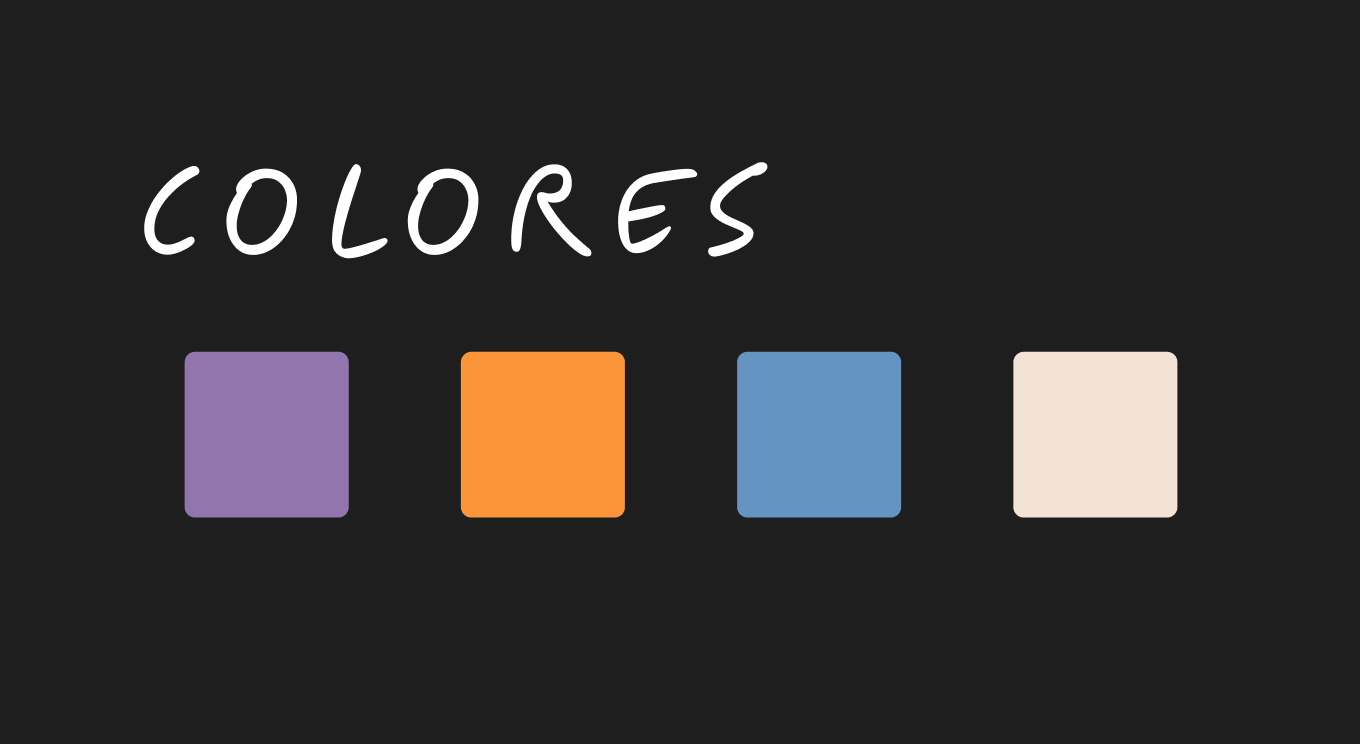
\includegraphics[width=7cm]{Colors.jpg}\par}
		\caption{Colores principales}
	\end{center}
\end{figure}

Como fuente, se opta por escoger la fuente \textit{Nunito Sans}, que proporciona Google. Se escoge porque es una fuente bastante estándar y legible para cualquier tipo de usuario.

\begin{figure}[H]
	\begin{center}
		{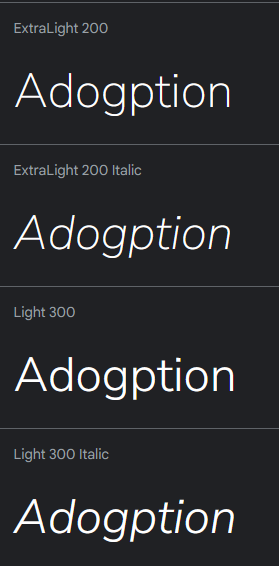
\includegraphics[width=7cm]{NunitoFont.png}\par}
		\caption{Fuente Nunito Sans}
	\end{center}
\end{figure}

\subsubsection{Nombre}

Como nombre de la aplicación,  se tiene en cuenta que inicialmente la aplicación está dirigida a la adopción de perros, así que se propone un juego de palabras. Uniendo las palabras \textit{Adoption} y \textit{Dog} que son la traducción de las palabras adopción y perro. Se decide que el nombre de la aplicación sea: \textbf{\textit{Adogption}}.

\subsubsection{Logo e iconos}

La última parte relacionada con el branding en este proyecto es la de generación de logos e iconos. En esta sección se incluye tanto el logo de la aplicación como los iconos que se han hecho para incluir dentro de la aplicación. Algunos de los iconos podrían finalmente no utilizarse.

La idea del logo es que se perciba claramente que la aplicación va sobre perros. Los corgis son unas de las razas más populares en el mundo, destacan por que es una raza muy amigable y muy querida dentro de la cultura pop, lo que la convierte en la cara perfecta para llamar la atención. Además del logo principal, hemos generado un logo animado con las letras de la aplicación para incluir en pantallas de carga o en otros lugares. Por último, se han hecho algunos iconos por defecto.



\begin{figure}[H]
   	\begin{minipage}{0.48\textwidth}
		\begin{center}
			{
\includegraphics[width=6cm]{Logo1.png}\par}
			\caption{Logo}
		\end{center}  
	\end{minipage}\hfill
   	\begin{minipage}{0.48\textwidth}
		\begin{center}
			{
\includegraphics[width=7cm]{ADOGPTIONFIXED.png}\par}
			\caption{Logo animado}
		\end{center}  
	\end{minipage}\hfill
\end{figure}


\begin{figure}[H]
   	\begin{minipage}{0.48\textwidth}
		\begin{center}
			{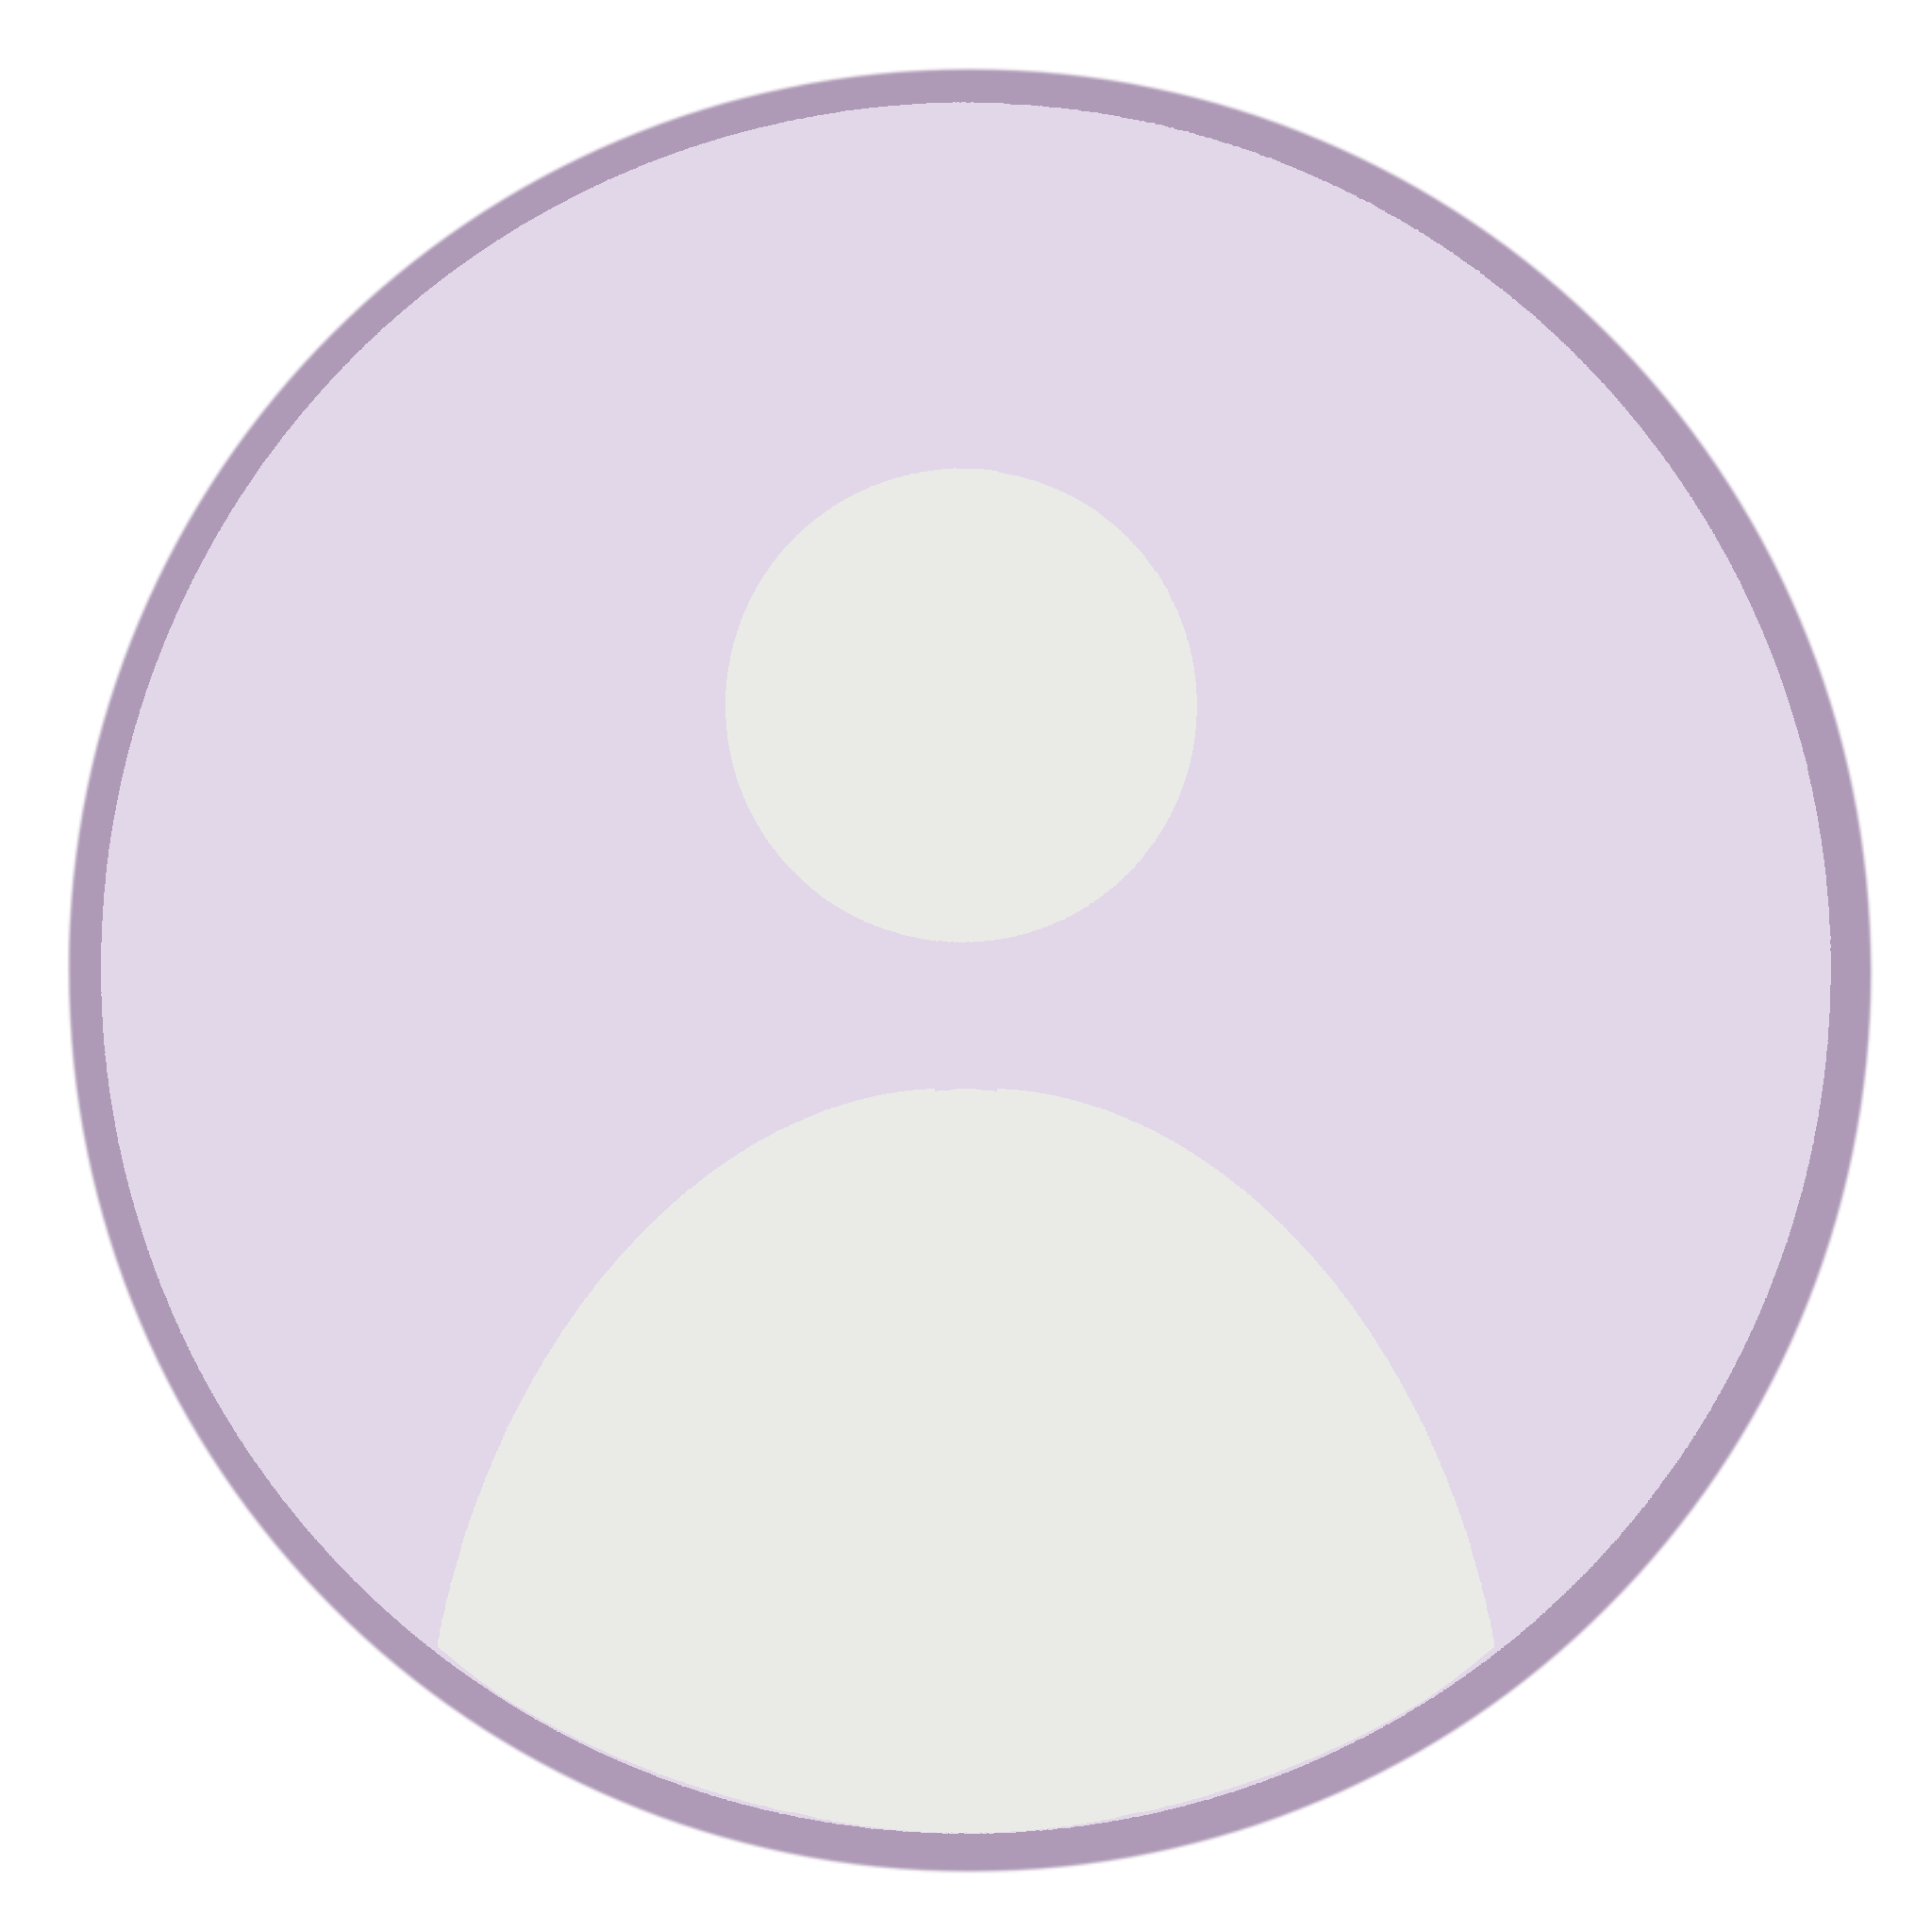
\includegraphics[width=6cm]{EMPTYUSER.png}\par}
			\caption{Icono por defecto para usuario}
		\end{center}  
	\end{minipage}\hfill
   	\begin{minipage}{0.48\textwidth}
		\begin{center}
			{
\includegraphics[width=6cm]{EMPTYDOG.png}\par}
			\caption{Icono por defecto para perro}
		\end{center}  
	\end{minipage}\hfill
\end{figure}

\subsubsection{Diseños}

En esta sección se incluyen todos los diseños realizados en \textit{Figma} para las pantallas de la aplicación. Se incluyen todas las páginas principales y componentes relevantes para el desarrollo de la aplicación.


\begin{figure}[H]
   	\begin{minipage}{0.48\textwidth}
		\begin{center}
			{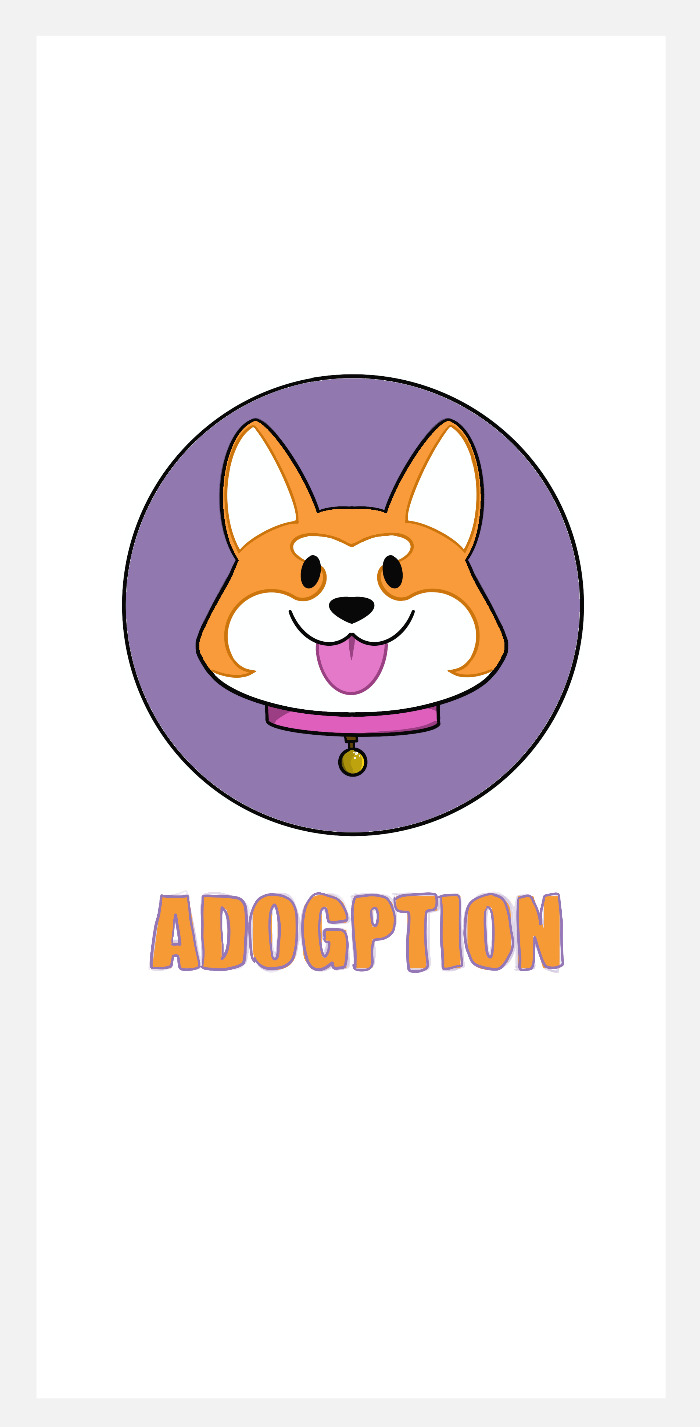
\includegraphics[height=8cm]{SplashScreen.jpg}\par}
			\caption{Splashscreen}
			\medskip
			\small
			Página de carga entre pantallas.
		\end{center}  
	\end{minipage}\hfill
   	\begin{minipage}{0.48\textwidth}
		\begin{center}
			{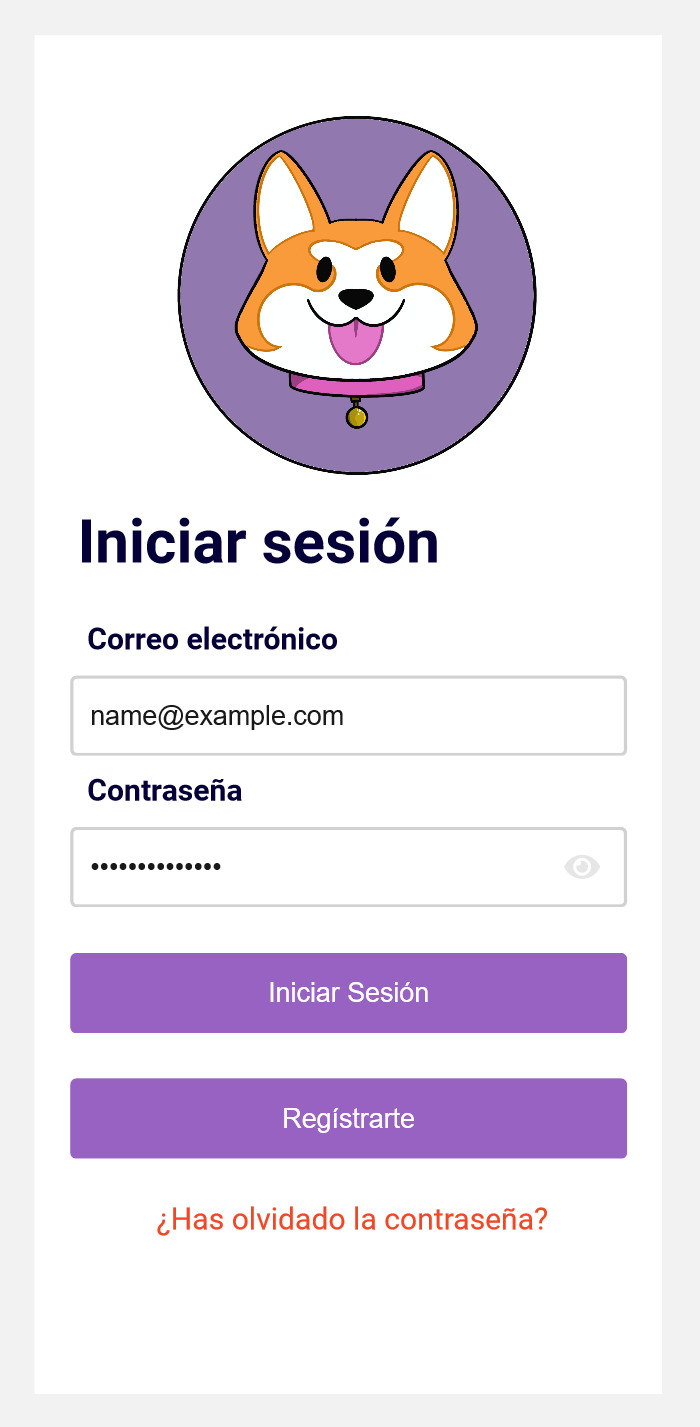
\includegraphics[height=8cm]{Login.jpg}\par}
			\caption{Login}
			\medskip
			\small
			Página de inicio de sesión.
		\end{center}  
	\end{minipage}\hfill
\end{figure}


\begin{figure}[H]
   	\begin{minipage}{0.48\textwidth}
		\begin{center}
			{
\includegraphics[height=8cm, width=4cm]{White.png}\par}
			\caption{User register}
			\medskip
			\small
			Página de registro de usuario.
		\end{center}  
	\end{minipage}\hfill
   	\begin{minipage}{0.48\textwidth}
		\begin{center}
			{
\includegraphics[height=8cm, width=4cm]{White.png}\par}
			\caption{Company register}
			\medskip
			\small
			Página de registro de protectora.
		\end{center}  
	\end{minipage}\hfill
\end{figure}

\begin{figure}[H]
   	\begin{minipage}{0.48\textwidth}
		\begin{center}
			{
\includegraphics[height=8cm, width=4cm]{White.png}\par}
			\caption{User homepage}
			\medskip
			\small
			Página de inicio de usuario.
		\end{center}  
	\end{minipage}\hfill
   	\begin{minipage}{0.48\textwidth}
		\begin{center}
			{
\includegraphics[height=8cm, width=4cm]{White.png}\par}
			\caption{Company homepage}
			\medskip
			\small
			Página de inicio de protectora.
		\end{center}  
	\end{minipage}\hfill
\end{figure}

\begin{figure}[H]
   	\begin{minipage}{0.48\textwidth}
		\begin{center}
			{
\includegraphics[height=8cm, width=4cm]{White.png}\par}
			\caption{Dog list}
			\medskip
			\small
			Página de lista para perros.
		\end{center}  
	\end{minipage}\hfill
   	\begin{minipage}{0.48\textwidth}
		\begin{center}
			{
\includegraphics[height=8cm, width=4cm]{White.png}\par}
			\caption{User list}
			\medskip
			\small
			Página de lista para usuarios.
		\end{center}  
	\end{minipage}\hfill
\end{figure}


\begin{figure}[H]
   	\begin{minipage}{0.48\textwidth}
		\begin{center}
			{
\includegraphics[height=8cm, width=4cm]{White.png}\par}
			\caption{User profile}
			\medskip
			\small
			Página de perfil de usuario. Se muestran botones de edición si es necesario.
		\end{center}  
	\end{minipage}\hfill
   	\begin{minipage}{0.48\textwidth}
		\begin{center}
			{
\includegraphics[height=8cm, width=4cm]{White.png}\par}
			\caption{Dog profile}
			\medskip
			\small
			Página de perfil de perro. Se muestran botones de edición si es necesario.
		\end{center}  
	\end{minipage}\hfill
\end{figure}

\begin{figure}[H]
   	\begin{minipage}{0.48\textwidth}
		\begin{center}
			{
\includegraphics[height=8cm, width=4cm]{White.png}\par}
			\caption{Chats page}
			\medskip
			\small
			Página de chats.
		\end{center}  
	\end{minipage}\hfill
   	\begin{minipage}{0.48\textwidth}
		\begin{center}
			{
\includegraphics[height=8cm, width=4cm]{White.png}\par}
			\caption{Chat room}
			\medskip
			\small
			Página de mensajes.
		\end{center}  
	\end{minipage}\hfill
\end{figure}

\begin{figure}[H]
   	\begin{minipage}{0.48\textwidth}
		\begin{center}
			{
\includegraphics[height=8cm, width=4cm]{White.png}\par}
			\caption{Maps list}
			\medskip
			\small
			Página de mapa con lista de usuarios.
		\end{center}  
	\end{minipage}\hfill
   	\begin{minipage}{0.48\textwidth}
		\begin{center}
			{
\includegraphics[height=8cm, width=4cm]{White.png}\par}
			\caption{Recover password}
			\medskip
			\small
			Página de recuperación de contraseña.
		\end{center}  
	\end{minipage}\hfill
\end{figure}

\begin{figure}[H]
   	\begin{minipage}{0.48\textwidth}
		\begin{center}
			{
\includegraphics[height=8cm, width=4cm]{White.png}\par}
			\caption{Edit user}
			\medskip
			\small
			Página de edición de usuario
		\end{center}  
	\end{minipage}\hfill
   	\begin{minipage}{0.48\textwidth}
		\begin{center}
			{
\includegraphics[height=8cm, width=4cm]{White.png}\par}
			\caption{Edit dog}
			\medskip
			\small
			Página de edición de perro
		\end{center}  
	\end{minipage}\hfill
\end{figure}

\begin{figure}[H]
   	\begin{minipage}{0.48\textwidth}
		\begin{center}
			{
\includegraphics[height=8cm, width=4cm]{White.png}\par}
			\caption{Admin homepage}
			\medskip
			\small
			Página de inicio de administrador
		\end{center}  
	\end{minipage}\hfill
   	\begin{minipage}{0.48\textwidth}
		\begin{center}
			{
\includegraphics[height=8cm, width=4cm]{White.png}\par}
			\caption{Verify user}
			\medskip
			\small
			Pop up para verificar usuario
		\end{center}  
	\end{minipage}\hfill
\end{figure}


\begin{figure}[H]
   	\begin{minipage}{0.48\textwidth}
		\begin{center}
			{
\includegraphics[height=8cm, width=4cm]{White.png}\par}
			\caption{Side menu}
			\medskip
			\small
			Menú lateral con páginas disponibles
		\end{center}  
	\end{minipage}\hfill
\end{figure}




\subsection{Arquitectura de sistema}
Definicion de modulos?
Tengo mas de 100 clases? que hago aqui


% Implementación
\newpage
\section{Implementación}

% Implementación
\newpage
\section{Conclusiones}
\subsection{Objetivos conseguidos}

En este apartado volvemos a repasar todos los requisitos funcionales que se plantearon al inicio para comprobar si se han conseguido o no.

% Objetivo 1
\begin{table}[H]
	\captionsetup{width=0.95\linewidth}%
   	\captionsetup{singlelinecheck=false}%
	\captionsetup{font=bf}
	\caption{Objetivo 1}
	\begin{tabular}{ | m{3cm} | m{10cm} | }
		\hline \cellcolor{lightgray}\textbf{Título} & \cellcolor{gray} \textcolor{white}{\textit{Registro de usuarios con diferentes roles}}  \\ \hline
		\cellcolor{lightgray}\textbf{Tipo} & Obligatorio \\ \hline
		\cellcolor{lightgray}\textbf{Conseguido} & Si \\ \hline
		\cellcolor{lightgray}\textbf{Explicación} & Explicacion de que se ha hecho o que no se ha hecho.  \\ \hline
	\end{tabular}
\end{table} 

% Objetivo 2
\begin{table}[H]
	\captionsetup{width=0.95\linewidth}%
   	\captionsetup{singlelinecheck=false}%
	\captionsetup{font=bf}
	\caption{Objetivo 2}
	\begin{tabular}{ | m{3cm} | m{10cm} | }
		\hline \cellcolor{lightgray}\textbf{Título} & \cellcolor{gray} \textcolor{white}{\textit{Registro de caninos}}  \\ \hline
		\cellcolor{lightgray}\textbf{Tipo} & Obligatorio \\ \hline
		\cellcolor{lightgray}\textbf{Conseguido} & Si \\ \hline
		\cellcolor{lightgray}\textbf{Explicación} & Explicacion de que se ha hecho o que no se ha hecho.  \\ \hline
	\end{tabular}
\end{table} 

% Objetivo 3
\begin{table}[H]
	\captionsetup{width=0.95\linewidth}%
   	\captionsetup{singlelinecheck=false}%
	\captionsetup{font=bf}
	\caption{Objetivo 3}
	\begin{tabular}{ | m{3cm} | m{10cm} | }
		\hline \cellcolor{lightgray}\textbf{Título} & \cellcolor{gray} \textcolor{white}{\textit{Listas de caninos con filtros y búsqueda}}  \\ \hline
		\cellcolor{lightgray}\textbf{Tipo} & Obligatorio \\ \hline
		\cellcolor{lightgray}\textbf{Conseguido} & Si \\ \hline
		\cellcolor{lightgray}\textbf{Explicación} & Explicacion de que se ha hecho o que no se ha hecho.  \\ \hline
	\end{tabular}
\end{table} 

% Objetivo 4
\begin{table}[H]
	\captionsetup{width=0.95\linewidth}%
   	\captionsetup{singlelinecheck=false}%
	\captionsetup{font=bf}
	\caption{Objetivo 4}
	\begin{tabular}{ | m{3cm} | m{10cm} | }
		\hline \cellcolor{lightgray}\textbf{Título} & \cellcolor{gray} \textcolor{white}{\textit{Listas de usuarios con búsqueda}}  \\ \hline
		\cellcolor{lightgray}\textbf{Tipo} & Obligatorio \\ \hline
		\cellcolor{lightgray}\textbf{Conseguido} & Si \\ \hline
		\cellcolor{lightgray}\textbf{Explicación} & Explicacion de que se ha hecho o que no se ha hecho.  \\ \hline
	\end{tabular}
\end{table} 

% Objetivo 5
\begin{table}[H]
	\captionsetup{width=0.95\linewidth}%
   	\captionsetup{singlelinecheck=false}%
	\captionsetup{font=bf}
	\caption{Objetivo 5}
	\begin{tabular}{ | m{3cm} | m{10cm} | }
		\hline \cellcolor{lightgray}\textbf{Título} & \cellcolor{gray} \textcolor{white}{\textit{Sección de perros favoritos}}  \\ \hline
		\cellcolor{lightgray}\textbf{Tipo} & Obligatorio \\ \hline
		\cellcolor{lightgray}\textbf{Conseguido} & Si \\ \hline
		\cellcolor{lightgray}\textbf{Explicación} & Explicacion de que se ha hecho o que no se ha hecho.  \\ \hline
	\end{tabular}
\end{table} 

% Objetivo 6
\begin{table}[H]
	\captionsetup{width=0.95\linewidth}%
   	\captionsetup{singlelinecheck=false}%
	\captionsetup{font=bf}
	\caption{Objetivo 6}
	\begin{tabular}{ | m{3cm} | m{10cm} | }
		\hline \cellcolor{lightgray}\textbf{Título} & \cellcolor{gray} \textcolor{white}{\textit{Sistema de mensajería entre usuarios}}  \\ \hline
		\cellcolor{lightgray}\textbf{Tipo} & Obligatorio \\ \hline
		\cellcolor{lightgray}\textbf{Conseguido} & Si \\ \hline
		\cellcolor{lightgray}\textbf{Explicación} & Explicacion de que se ha hecho o que no se ha hecho.  \\ \hline
	\end{tabular}
\end{table} 

% Objetivo 7
\begin{table}[H]
	\captionsetup{width=0.95\linewidth}%
   	\captionsetup{singlelinecheck=false}%
	\captionsetup{font=bf}
	\caption{Objetivo 7}
	\begin{tabular}{ | m{3cm} | m{10cm} | }
		\hline \cellcolor{lightgray}\textbf{Título} & \cellcolor{gray} \textcolor{white}{\textit{Geolocalización y mapas con  resultados}}  \\ \hline
		\cellcolor{lightgray}\textbf{Tipo} & Obligatorio \\ \hline
		\cellcolor{lightgray}\textbf{Conseguido} & Si \\ \hline
		\cellcolor{lightgray}\textbf{Explicación} & Explicacion de que se ha hecho o que no se ha hecho.  \\ \hline 
	\end{tabular}
\end{table} 

% Objetivo 8
\begin{table}[H]
	\captionsetup{width=0.95\linewidth}%
   	\captionsetup{singlelinecheck=false}%
	\captionsetup{font=bf}
	\caption{Objetivo 8}
	\begin{tabular}{ | m{3cm} | m{10cm} | }
		\hline \cellcolor{lightgray}\textbf{Título} & \cellcolor{gray} \textcolor{white}{\textit{Actualizar datos de caninos}}  \\ \hline
		\cellcolor{lightgray}\textbf{Tipo} & Obligatorio \\ \hline
		\cellcolor{lightgray}\textbf{Conseguido} & Si \\ \hline
		\cellcolor{lightgray}\textbf{Explicación} & Explicacion de que se ha hecho o que no se ha hecho.  \\ \hline
	\end{tabular}
\end{table} 

% Objetivo 9
\begin{table}[H]
	\captionsetup{width=0.95\linewidth}%
   	\captionsetup{singlelinecheck=false}%
	\captionsetup{font=bf}
	\caption{Objetivo 9}
	\begin{tabular}{ | m{3cm} | m{10cm} | }
		\hline \cellcolor{lightgray}\textbf{Título} & \cellcolor{gray} \textcolor{white}{\textit{Actualizar datos de usuarios}}  \\ \hline
		\cellcolor{lightgray}\textbf{Tipo} & Obligatorio \\ \hline
		\cellcolor{lightgray}\textbf{Conseguido} & Si \\ \hline
		\cellcolor{lightgray}\textbf{Explicación} & Explicacion de que se ha hecho o que no se ha hecho.  \\ \hline
	\end{tabular}
\end{table} 

% Objetivo 10
\begin{table}[H]
	\captionsetup{width=0.95\linewidth}%
   	\captionsetup{singlelinecheck=false}%
	\captionsetup{font=bf}
	\caption{Objetivo 10}
	\begin{tabular}{ | m{3cm} | m{10cm} | }
		\hline \cellcolor{lightgray}\textbf{Título} & \cellcolor{gray} \textcolor{white}{\textit{Barra de búsqueda de direcciones}}  \\ \hline
		\cellcolor{lightgray}\textbf{Tipo} & Opcional \\ \hline
		\cellcolor{lightgray}\textbf{Conseguido} & Si \\ \hline
		\cellcolor{lightgray}\textbf{Explicación} & Explicacion de que se ha hecho o que no se ha hecho.  \\ \hline
	\end{tabular}
\end{table}

% Objetivo 11
\begin{table}[H]
	\captionsetup{width=0.95\linewidth}%
   	\captionsetup{singlelinecheck=false}%
	\captionsetup{font=bf}
	\caption{Objetivo 11}
	\begin{tabular}{ | m{3cm} | m{10cm} | }
		\hline \cellcolor{lightgray}\textbf{Título} & \cellcolor{gray} \textcolor{white}{\textit{Tema oscuro en la aplicación}}  \\ \hline
		\cellcolor{lightgray}\textbf{Tipo} & Opcional \\ \hline
		\cellcolor{lightgray}\textbf{Conseguido} & No \\ \hline
		\cellcolor{lightgray}\textbf{Explicación} & Explicacion de que se ha hecho o que no se ha hecho.  \\ \hline
	\end{tabular}
\end{table}  

% Objetivo 12
\begin{table}[H]
	\captionsetup{width=0.95\linewidth}%
   	\captionsetup{singlelinecheck=false}%
	\captionsetup{font=bf}
	\caption{Objetivo 12}
	\begin{tabular}{ | m{3cm} | m{10cm} | }
		\hline \cellcolor{lightgray}\textbf{Título} & \cellcolor{gray} \textcolor{white}{\textit{Blog}}  \\ \hline
		\cellcolor{lightgray}\textbf{Tipo} & Opcional \\ \hline
		\cellcolor{lightgray}\textbf{Conseguido} & No \\ \hline
		\cellcolor{lightgray}\textbf{Explicación} & Explicacion de que se ha hecho o que no se ha hecho.  \\ \hline
	\end{tabular}
\end{table}  

% Objetivo 13
\begin{table}[H]
	\captionsetup{width=0.95\linewidth}%
   	\captionsetup{singlelinecheck=false}%
	\captionsetup{font=bf}
	\caption{Objetivo 13}
	\begin{tabular}{ | m{3cm} | m{10cm} | }
		\hline \cellcolor{lightgray}\textbf{Título} & \cellcolor{gray} \textcolor{white}{\textit{Compartir perros a través de enlace}}  \\ \hline
		\cellcolor{lightgray}\textbf{Tipo} & Opcional \\ \hline
		\cellcolor{lightgray}\textbf{Conseguido} & Si \\ \hline
		\cellcolor{lightgray}\textbf{Explicación} & Explicacion de que se ha hecho o que no se ha hecho.  \\ \hline
	\end{tabular}
\end{table}  

% Objetivo 14
\begin{table}[H]
	\captionsetup{width=0.95\linewidth}%
   	\captionsetup{singlelinecheck=false}%
	\captionsetup{font=bf}
	\caption{Objetivo 14}
	\begin{tabular}{ | m{3cm} | m{10cm} | }
		\hline \cellcolor{lightgray}\textbf{Título} & \cellcolor{gray} \textcolor{white}{\textit{Mandar imágenes dentro del chat}}  \\ \hline
		\cellcolor{lightgray}\textbf{Tipo} & Opcional \\ \hline
		\cellcolor{lightgray}\textbf{Conseguido} & Si \\ \hline
		\cellcolor{lightgray}\textbf{Explicación} & Explicacion de que se ha hecho o que no se ha hecho.  \\ \hline
	\end{tabular}
\end{table} 

\subsection{Próximos pasos}

Tras repasar la lista de objetivos, vemos que la aplicación permite realizar todas las funcionalidades obligatorias y necesarias para un correcto uso de la aplicación. Sin embargo, algunos de los objetivos opcionales se han quedado sin realizar. Para próximas iteraciones podemos añadir como obligatorias las funcionalidades que se han quedado sin implementar en esta primera versión. 

Para responder a la pregunta de porque no se han podido implementar todas las funcionalidades, es debido a que hubo un retraso en el desarrollo. Este retraso es fruto de la dificultad a la hora de implementar ciertas funcionalidades, como el chat en tiempo real o la lista dinámica en el mapa. 

Para futuras iteraciones, se han planteado propuestas para añadir valor a la aplicación y mejorar la experiencia de uso del usuario.

\begin{itemize}
	\item Añadir la posibilidad de crear listas con filtros a las protectoras.
	\item Permitir subir múltiples imágenes para los perros dados de alta, además de vídeos y poder generar un albúm por cada perro.
	\item Permitir asignar a un usuario como adoptante/acogedor de un perro, además de indicar en el perfil del perro quien es su adoptante/acogedor.
	\item Sumar las funcionalidades mandar mensajes de audios y vídeos dentro del chat
	\item Añadir como atributos opcionales de usuario distintas redes sociales e incluso el número de teléfono.
	\item Permitir compartir perfiles de protectoras.
\end{itemize}

 

\subsection{Valoración personal}


% Bibliografía
\newpage
\section{Bibliografía}

% Bibliografía
\newpage
\section{Anexos}

\printindex
\end{document}